\chapter{Production de mots-clés de bout-en-bout} \label{chap:kw_production}

Ce chapitre présente les méthodes de production de mots-clés de l'état de l'art de bout-en-bout, qui constituent l'élément principal de ce travail de thèse. 
Nous commencerons par présenter les composants de ces méthodes auxquels nous feront référence dans la partie état de l'art.

\section{Principes fondamentaux des réseaux de neurones}
% Fondements sur les réseaux de neurones

Nous présentons dans cette section les concepts nécessaires à la bonne compréhension des méthodes de production de mots-clés de bout-en-bout.
Nous décrivons d'abord en détail les réseaux de neurones, ensuite les plongements de mots (\foreign{word embeddings}) utilisés pour représenter les mots du langage naturel, et enfin le paradigme encodeur-décodeur qui permet de traiter du texte de longueur variable en entrée et en sortie des réseaux de neurones.

Contrairement aux méthodes en chaîne de traitement décrites dans la section~\ref{sec:methode-en-chaine-de-traitement}, les méthodes de bout-en-bout, qui utilisent le paradigme encodeur-décodeur, se passent de l'identification des candidats ainsi que du choix des caractéristiques des mots-clés qui serviront à les pondérer.
En effet, les méthodes que nous décrivons dans ce chapitre utilisent des réseaux de neurones profonds qui apprennent à extraire automatiquement les descripteurs  les plus pertinents.
%L'apprentissage profond, permet de laisser le modèle extraire les descripteurs de manière automatique au lieu de les définir à la main, ce qui nécessite des connaissances expertes. Mais cela est difficile à interpreter, tout un pan de la recherche s'intéresse à expliquer ces méthodes (blackbox nlp)~\cite{}.


\subsection{Réseaux de neurones}
\label{sub:neural_network}

\begin{figure}
    \centering
    %Heavily inspired from https://texample.net/tikz/examples/neural-network/

\begin{tikzpicture}[shorten >=1pt,->,draw=black!50]
    \def\myscale{1.5}
    \tikzstyle{neuron}=[circle,fill=black!25,minimum size=17*\myscale,inner sep=0cm]
    \tikzstyle{input neuron}=[neuron, fill=color1!60];
    \tikzstyle{hidden neuron}=[neuron, fill=color0!60];
    \tikzstyle{output neuron}=[neuron, fill=color2!60];
    \tikzstyle{edge label}=[above=-.025cm,sloped,scale=.4*\myscale,black!60]
    \tikzstyle{label}=[scale=.75*\myscale, text width=2cm, align=center]

    \def\layersep{2.5*\myscale}
    \def\ninput{2}
    \def\nlayerone{3}
    \def\nlayertwo{2}
    \def\noutput{2}

    % Draw the input layer nodes
    \foreach \name / \y in {1,...,\ninput}
    % This is the same as writing \foreach \name / \y in {1/1,2/2,3/3,4/4}
        \node[input neuron] (I-\name) at (0,-\y*\myscale) {};


    % Draw the hidden layer nodes
    \foreach \name / \y in {1,...,\nlayerone}
        \path[yshift=.5*\myscale cm]
            node[hidden neuron] (H1-\name) at (1*\layersep,-\y*\myscale) {};

    \foreach \name / \y in {1,...,\nlayertwo}
        \path[yshift=.0*\myscale cm]
            node[hidden neuron] (H2-\name) at (2*\layersep,-\y*\myscale) {};

    % Draw the output layer node
    \foreach \name / \y in {1,...,\noutput}
        \path[yshift=0*\myscale cm]
            node [output neuron] (O-\name) at (3*\layersep,-\y*\myscale) {};

    % Connect every node in the input layer with every node in the
    % hidden layer.
    
    %\foreach \source in {1,...,\ninput}
    %    \foreach \dest in {1,...,\nlayerone}
    %        \draw[->] (I-\source) -- node [edge label, pos={.28-}] {$W^1_{\source,\dest}$} (H1-\dest);
    
    \def\layerout{1}
    \def\source{1}
    \foreach \dest / \n in {1/.2,2/.25,3/.235}
        \draw[->] (I-\source) -- node [edge label, pos={\n}] {$W^\layerout_{\source,\dest}$} (H\layerout-\dest);
    \def\source{2}
    \foreach \dest / \n in {1/.17,2/.285,3/.26}
        \draw[->] (I-\source) -- node [edge label, pos={\n}] {$W^\layerout_{\source,\dest}$} (H\layerout-\dest);


    \def\layerout{2} % modify this
    \pgfmathtruncatemacro{\layerin}{\layerout - 1}
    \def\source{1} % modify this
    \foreach \dest / \n in {1/.2,2/.26} % modify this
        \draw[->] (H\layerin-\source) -- node [edge label, pos={\n}] {$W^\layerout_{\source,\dest}$} (H\layerout-\dest);
    \def\source{2} % modify this
    \foreach \dest / \n in {1/.2,2/.25} % modify this
        \draw[->] (H\layerin-\source) -- node [edge label, pos={\n}] {$W^\layerout_{\source,\dest}$} (H\layerout-\dest);
    \def\source{3} % modify this
    \foreach \dest / \n in {1/.23,2/.3} % modify this
        \draw[->] (H\layerin-\source) -- node [edge label, pos={\n}] {$W^\layerout_{\source,\dest}$} (H\layerout-\dest);

    % Connect every node in the hidden layer with the output layer
    \def\layerout{3} % modify this
    \pgfmathtruncatemacro{\layerin}{\layerout - 1}
    \foreach \source in {1,...,\nlayertwo}
        \foreach \dest in {1,...,\noutput}
            \draw[->] (H\layerin-\source) -- node [edge label, pos={.20+(1-Mod(\dest,2))*.05}] {$W^\layerout_{\source,\dest}$} (O-\dest);

    % Annotate the layers
    \node[label, below=.1cm of I-\ninput] (I-label) {Entrée};

    \node[draw, dashed, rounded corners,fill=none, fit=(H1-1) (H1-\nlayerone)] (H1) {};
    \node[label, below=.1cm of H1] (H1-label) {Première couche};

    \node[draw, dashed, rounded corners,fill=none, fit=(H2-1) (H2-\nlayertwo)] (H2) {};
    \node[label, below=.1cm of H2] (H2-label) {Seconde couche};

    \node[draw, dashed, rounded corners,fill=none, fit=(O-1) (O-\noutput)] (O) {};
    \node[label, below=.1cm of O] (O-label) {Couche de sortie};

    \node[draw, dashed, rounded corners,fill=none, fit=(H1) (H1-label) (H2) (H2-label)] (H) {};
    \node[label, text width=10cm, below=.1cm of H] (H-label) {Couches cachées};

\end{tikzpicture}
    \caption{Représentation graphique d'un réseau de neurones à 2 couches. Les flèches représentent les poids des matrices $W^k$. Les biais $b^k$ ne sont pas représentés.}
    \label{fig:ex_nn_simple}
\end{figure}
% https://texample.net/tikz/examples/neural-network/

Les réseaux de neurones servent à modéliser des fonctions complexes, qui peuvent être non linéaires.
%
D'un point de vue mathématique, il s'agit de modéliser une fonction $f$ qui prend une entrée $X$ et retourne une sortie (une prédiction) $\hat{Y} = f(X)$.
%
Ici, $X \in M_{1,m}(\mathds{R})$ et $\hat{Y} \in M_{1,n}(\mathds{R})$ sont des vecteurs de taille $m$ et $n$ respectivement.
%
Ces vecteurs représentent le nombre de paramètres d'entrée de la fonction $f$.
%
%Par exemple, un modèle qui prédit le prix d'une maison en fonction de sa surface et du nombre de fenêtres aura 2 entrées et une sortie.


Un réseau de neurones simple (également appelé perceptron mono-couche) est défini par l'équation~\ref{eq:simple_nn} ci-dessous, dans laquelle $W$ est une matrice de poids $W \in M_{m, n}(\mathds{R})$ et $b$ un vecteur de biais $b \in M_{1,m}(\mathds{R})$.
%
\begin{align}
    \hat{Y} = f(X) = \sigma (b + W * X) \label{eq:simple_nn}
\end{align}


La fonction $\sigma$ est une fonction dite d'activation.
Elle est inspirée de l'activation des neurones dans le cerveau humain.
L'information d'un neurone passe à la couche suivante si le neurone est activé (c'est-à-dire si sa valeur est assez élevée).
Les fonctions Sigmoïde (voir équation~\ref{eq:sigmoide}) et Rectified Linear Unit (ReLU) (voir équation~\ref{eq:relu}) sont généralement utilisées pour $\sigma$.
%Cette fonction est généralement la fonction sigmoïde (équation~\ref{eq:sigmoide}), Rectified Linear Unit (ReLU) (équation~\ref{eq:relu}), ou tangente hyperbolique ($\text{tanh}$). \todo{comment choisir cette fonction ?}

\begin{gather}
    \sigma(x) = \frac{1}{1+e^{-x}} \label{eq:sigmoide} \\
    \textsc{ReLu}(x) = \text{max}(0, x) \label{eq:relu}
\end{gather}

%\begin{figure}\centering
%    \begin{tikzpicture}\begin{axis}[xmin=-5, xmax=5, ymin=-2, ymax=2]
%        \addplot {1/(1+e^(-x))};
%        \addplot {tanh(x)};
%        \addplot {max(x, 0};
%    \end{axis}\end{tikzpicture}
%    \caption{Caption} \label{fig:my_label}
%\end{figure}

Un réseau de neurones à une couche (perceptron mono-couche) ne peut modéliser que des fonctions linéaires, et ne pourra jamais modéliser une fonction telle que la fonction XOR par exemple~\cite{minsky_perceptrons_1988}.
Pour gagner en expressivité, des couches de neurones sont ajoutées (voir figure~\ref{fig:ex_nn_simple}). Un tel réseau de neurones est aussi appelé perceptron multicouche.
%
Un perceptron mono ou multicouche dénote un réseau de neurones à propagation avant (\foreign{feed forward neural network}) où chaque couche est entièrement connectée à la suivante.

En utilisant les perceptrons multicouche, il est possible de modéliser des fonctions plus complexes.
Dans ce cas, chaque couche utilise la sortie de la couche précédente comme entrée (voir équation~\ref{eq:multi_nn}).
La couche \num{0} représente l'entrée du réseau, $k$ représente une couche intermédiaire et $n$ la couche de sortie.
Les matrices $W$ (et leur vecteurs de biais) définissent la taille de chaque couche (c'est-à-dire le nombre de neurones).
En effet, une matrice de taille $n*m$ (et un vecteur $b$ de taille $m$) définit une couche de taille $m$, $n$ étant conditionné par la taille de la couche précédente.
%
\begin{equation}\label{eq:multi_nn}
  \begin{split}
    h^0 & = X \\
    h^k & = \sigma(b^k + W^k * h^{k-1}) \\
    \hat{Y} & = h^n
  \end{split}
\end{equation}

Entraîner le réseau de neurones $f$ consiste à modifier les paramètres du modèle $\theta$ (matrices de poids $W^k$ et $b^k$) afin de minimiser l'erreur de prédiction. Cette erreur est définie par une fonction de coût (\emph{loss function}) $\mathcal{L}$ (voir équation~\ref{eq:loss}) calculé grâce à une prédiction $\hat{Y} = f(X)$ et une vérité terrain $Y$.
Le but de l'entraînement est de minimiser cette fonction de coût pour tous les exemples d'un jeu de données, dénoté par l'équation~\ref{eq:loss_dataset}.
%
\begin{gather} 
    \text{erreur} = \mathcal{L}(\hat{Y}, Y) = \mathcal{L}(f(X, \theta), Y) \label{eq:loss} \\
    \text{min}_\theta \sum_{(x, y) \in \mathcal{D}} \mathcal{L}(f(x, \theta), y) \label{eq:loss_dataset}
\end{gather}

L'algorithme utilisé pour minimiser la fonction de coût dans le cadre des réseaux de neurones est la descente de gradient~\cite{curry_method_1944} (Gradient Descent).
Le gradient de la fonction de coût donne la direction dans laquelle modifier les paramètres (ici les poids du réseau de neurones) pour minimiser ce coût.
Cet algorithme calcule le gradient avec tous les exemples du jeu de données puis met à jour les poids du réseau; ce processus est donc très long. Pour pallier cette lenteur, la descente de gradient par minibatch calcule le gradient à l'aide d'un nombre fixe d'exemples qui fait un compromis entre temps de calcul et utilisation d'un grand nombre d'exemples.
% figure 
%Cet algorithme utilise le fait que la fonction de coût et le réseau de neurones soient dérivables pour calculer le gradient de l'erreur et modifier les poids par rétro-propagation pour minimiser l'erreur.

Les réseaux de neurones que nous venons de décrire fonctionnent avec une entrée de taille fixe $X$; or dans le cas du texte, les entrées sont des séquences de mots de longueur variable, et n'ont donc pas de longueur fixe. Nous présentons dans la suite de cette section une architecture permettant de traiter les entrées de longueur variable.

\subsection{Encodage de séquences (encodeur)}
\label{sub:encoding}

\subsubsection{Représentation dense des mots}
\label{sec:word_embedding}

Les réseaux de neurones manipulent des vecteurs et des matrices de nombres. Le langage naturel étant constitué par des mots, il est nécessaire de transformer les mots en nombres.
Pour cela, un vocabulaire qui associe un nombre à chacun des mots est nécessaire. La méthode la plus simple est de considérer les mots les plus fréquents d'un ensemble de documents d'entraînement comme le vocabulaire $\mathcal{V}$.
Un vocabulaire de taille trop importante peut être difficile à modéliser et contiendra de nombreux hapax\footnote{Mots n'apparaissant qu'une seule fois.}. Il est donc courant de conserver les \num{50 000} mots les plus fréquents~\cite{meng_deep_2017,yuan_one_2020,ye_one2set_2021}.
%Plusieurs techniques sont utilisés pour représenter un document sous forme de vecteur à l'aide d'un tel vocabulaire.
%L'encodage \emph{one-hot}, crée un vecteur de la taille du vocabulaire $|\mathcal{V}|$ où chaque dimension représente la fréquence du mot correspondant dans le document. Cette méthode est peu efficiente en terme d'espace car le vecteur ainsi créé est creux (il contient une grande majorité de 0).

% exemple image
Aujourd'hui, les plongements de mots sont l'état de l'art en termes de représentation de mots. Ce sont des représentations denses apprises sur de grandes quantités de données qui modélisent les cooccurrences entre les mots: deux mots utilisés dans des contextes similaires auront des vecteurs similaires~\cite{mikolov_efficient_2013}.
Plusieurs méthodes ont été proposées pour pré-entraîner ces plongements.
Les méthodes précurseures word2vec~\cite{mikolov_efficient_2013} et gloVe~\cite{pennington_glove_2014} calculent des représentations fixes des mots. Leurs principales lacunes sont la prise en compte de mots hors du vocabulaire et la prise en compte de la polysémie. Pour prendre en compte les mots hors du vocabulaire, fastText~\cite{bojanowski_enriching_2017} apprend des plongements de n-grammes de caractères puis combine ceux-ci pour représenter le mot entier. Ensuite, pour traiter la polysémie, Elmo~\cite{peters_deep_2018} et Bert~\cite{devlin_bert_2019} calculent ces plongements en fonction du contexte des mots.
Il est aussi possible d'entraîner des plongements à l'aide d'une simple matrice de poids au début du réseau de neurones. Dans la tâche de génération de mots-clés, cette technique est la plus utilisée.


\subsubsection{Encodeurs}

Les encodeurs sont des réseaux de neurones qui permettent de traiter des séquences de longueur variable. Dans nos travaux ces séquences sont des documents textuels.
Les encodeurs prennent en entrée une séquence de vecteurs, ici des plongements de mots, et donnent en sortie un vecteur de pensée qui agrège l'information de la séquence d'entrée.

Il existe différents types de réseaux permettant d'encoder une séquence: les réseaux récurrents, les réseaux à convolution, les transformers, les réseaux à convolutions de graphes.
Nous nous intéresserons ici aux encodeurs récurrents, les plus utilisés pour la génération de mots-clés. 
Un encodeur récurrent est composé d'une ou plusieurs cellules récurrentes empilées.
Une cellule récurrente $\textsc{Rnn}$ encode une séquence selon l'équation~\ref{eq:rnn}.
%
\begin{equation}\label{eq:rnn}
\begin{split}
    h_t & = \textsc{Rnn}^e(x_{t}, h_{t-1}) \\
    \textsc{Rnn}^e(x_t, h_{t-1}) & = \text{tanh}(W_x * x_t + b_x + W_h * h_{t-1} + b_h)
\end{split}
\end{equation}

Dans l'équation~\ref{eq:rnn} $x_t$ représente le plongement du mot $t$, $h_t$ l'état caché au temps $t$ qui encode la sous-séquence d'entrée jusqu'au mot $t$, $W_x$ et $W_h$ des matrices de poids et $b_x$, $b_h$ les vecteurs de biais correspondants.
Le premier état caché $h_0$ est initialisé aléatoirement.
Ces réseaux sont dits récurrents car l'état caché $h_t$ est conditionné par les états cachés précédents.

Ce type d'encodeurs peut être utilisé pour entraîner un classifieur de documents en utilisant le dernier vecteur $h_t$, par exemple dans le cadre de la catégorisation de documents~\cite{wang_disconnected_2018} ou la détection de rumeurs~\cite{ma_detecting_2016}.
Il est aussi possible d'utiliser ces encodeurs pour entraîner des modèles d'annotation en séquence qui utilisent chaque représentation $h_t$ pour prédire l'étiquette du mot, par exemple dans le cadre de la reconnaissance d'entités nommées~\cite{zukov-gregoric_named_2018}.

% long dependence \todo{parler de ça}
% bidirectionnel
% oubli du début de  la séquence
Le principal écueil des réseaux récurrents est leur difficulté à garder en mémoire les dépendances à long terme.
Pour pallier ce problème, \citet{hochreiter_long_1997}  introduit les cellules LSTM (Long Short Term Memory).
Ces cellules récurrentes contiennent des \say{portes} qui leur permettent d'apprendre à sélectionner les informations à conserver ou à oublier à chaque temps $t$.
Elles donnent en sortie un état caché $h_t$ qui représente l'information pertinente au moment $t$ ainsi qu'un vecteur de contexte $C_t$ qui contient l'ensemble de l'information que la cellule a mémorisé.
Ce mécanisme de portes permet de prendre en compte les dépendances à long terme.
Cette cellule récurrente a été améliorée, notamment par les cellules récurrentes GRU (Gated Recurrent Unit)\cite{cho_learning_2014} qui simplifient les LSTM en combinant $h_t$ et $C_t$ en un unique vecteur ainsi qu'en diminuant le nombre de paramètres utilisés, ce qui en facilite l'entraînement.

Pour améliorer l'encodage des documents et la modélisation des dépendances à long terme, \citet{schuster_bidirectional_1997} présente des encodeurs bi-directionnels.
Ceux-ci sont composés de deux encodeurs qui encodent chacun la séquence dans un sens différent, du début à la fin et inversement.
Chacun de leurs états cachés sont ensuite concaténés pour n'en former qu'un. Ainsi, les états cachés de ce type d'encodeur représentent la séquence entière centrée sur le mot $t$.
%\say{You can't cram the meaning of a whole \%\&\!\$\# sentence into a single \$\&!\#* vector!} (R. Mooney).


\subsection{Génération de séquences (décodeur)}
\label{sub:decoding}

Le processus de décodage permet de générer une séquence de mots à partir d'un vecteur de pensée. Ce vecteur de pensée résulte généralement de l'encodage d'un document (cf. section~\ref{sub:encoding}).
Comme pour l'encodage, différents types de réseaux peuvent être utilisés: les réseaux récurrents, les réseaux à convolutions ou les transformers.
Nous nous intéressons ici aux réseaux récurrents, présentés dans la section~\ref{sub:encoding}.

Un décodeur récurrent est composé d'une ou plusieurs cellules récurrentes empilées.
La génération d'une séquence consiste à utiliser les états cachés $h_t$ pour prédire un mot, c'est-à-dire à produire une distribution de probabilités sur l'ensemble du vocabulaire puis à choisir le mot le plus probable.


Le processus de décodage est décrit par l'équation~\ref{eq:rnn_decodeur} avec $y_{t-1}$ le mot prédit précédemment, $h_{t-1}$ l'état caché précédent, $W_x$ et $W_h$ des matrices de poids et leurs biais correspondant $b_x$ et $b_h$.
Le premier mot $y_0$ est initialisé par un mot spécial; l'état caché $h_0$ est un vecteur de pensée.
Puis $p(y_t | y_{1,...,t-1},h_0)$ représente la distribution de probabilités sur le vocabulaire pour le mot $t$ en fonction des mots précédents et du vecteur de pensée $h_0$; $W_v$ et $b_v$ sont une matrice de poids et son biais.


\begin{equation} \label{eq:rnn_decodeur}
\begin{split}
    p(y_t | y_{1,...,t-1},h_0) & = \textsc{Softmax}(\sigma(W_v * h_t + b_v))\\
    h_t & = \textsc{Rnn}^d(y_{t-1}, h_{t-1}) \\
    \textsc{Rnn}^d(x_t, h_{t-1}) & = \text{tanh}(W_x * x_t + b_x + W_h * h_{t-1} + b_h)
    % p(Y) = \prod p(w_t|w_{t-1},...,w_0,h)
\end{split}
\end{equation}

La génération d'une séquence de mots s'effectue mot-à-mot grâce à un algorithme de décodage.
Chaque étape de décodage consiste à produire une distribution de probabilité sur le vocabulaire de sortie $p(y_t | y_{1,...,t-1},h_0)$ et à choisir un mot $\hat{y}_t$ qui maximise cette probabilité.
Cette étape est répétée jusqu'à ce qu'un mot spécial finissant la séquence soit généré ou que la séquence soit assez longue.

L'algorithme le plus simple consiste à choisir le mot le plus probable à chaque étape mais cela ne permet de générer qu'une seule séquence.
%
Dans le cadre de la génération de mots-clés il est souhaitable de générer plusieurs mots-clés et donc plusieurs séquences.
Pour cela, c'est l'algorithme de recherche en faisceau~\cite{ow_filtered_1988}, que nous schématisons dans la figure~\ref{fig:beam_search}, qui est utilisé.
Cet algorithme consiste à décoder un nombre fixe de séquences (deux dans le schéma).
Les étapes de décodage sont effectuées pour chacun des faisceaux et les mots à générer sont choisis dans l'ensemble des mots des faisceaux.
Dans la figure~\ref{fig:beam_search}, deux mots sont choisis au départ.
Une étape de décodage est ensuite effectuée pour les deux faisceaux.
\`A la troisième étape, le préfixe \texttt{ba} n'est pas conservé car les deux séquences les plus probables sont issues du préfixe \texttt{ab}.
\`A la fin de l'algorithme, deux séquences ont été générées: \texttt{aba} et \texttt{abb}.

\begin{figure}[ht!]
    \centering
    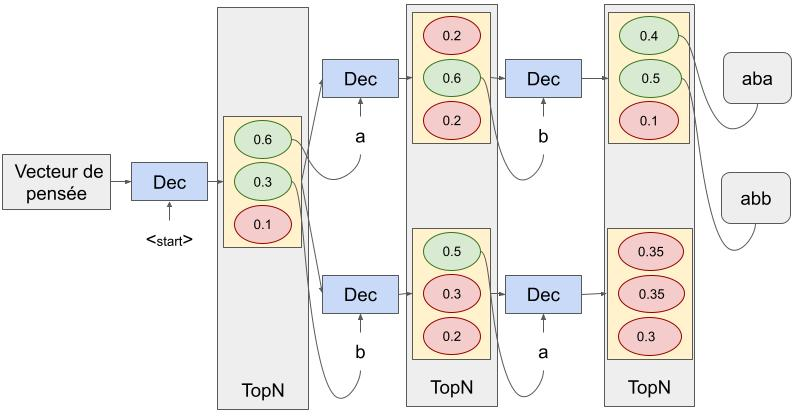
\includegraphics[scale=0.4]{2_production_mots_cles/Beam Search.jpg}
    \caption{Représentation schématique du processus de décodage grâce à l'algorithme de recherche en faisceau.}
    \label{fig:beam_search}
\end{figure}
\todo{refaire en tikz}

\`A l'inverse des algorithmes déterministes que nous avons décrits, notons l'existence des algorithmes d'échantillonnage. Ces algorithmes stochastiques choisissent les mots au hasard en fonction de leur probabilité. Les mots-clés générés par ces algorithmes ne sont donc pas reproductibles, ce qui dans le cadre de la production de mot-clés n'est pas souhaitable. Nous ne considérons donc pas cette technique.

\subsection{Paradigme encodeur-décodeur}\label{sub:paradigme_encodeur_decodeur}

Nous avons présenté dans les sections~\ref{sub:encoding} et \ref{sub:decoding} des moyens d'encoder des documents ainsi que des moyens de générer des séquences.
De nombreuses applications du traitement automatique de la langue nécessitent à la fois l'encodage d'une séquence et son décodage.
Par exemple dans le cadre de la traduction automatique, étant donnée une phrase en langue source, il faut la traduire dans une langue cible, c'est-à-dire qu'il faut encoder la phrase dans la langue source puis générer une phrase correspondante dans la langue cible.
Dans le cadre de la production de mots-clés, il faut générer un mot-clé en fonction d'un document.
Ainsi, le paradigme encodeur-décodeur introduit par \citet{sutskever_sequence_2014}, qui concatène un encodeur et un décodeur, permet de prendre en entrée une séquence de mots de longueur variable et de générer en sortie une autre séquence de mots de longueur variable.
Ce paradigme pallie la limite des réseaux de neurones présentés dans la section~\ref{sub:neural_network} (perceptrons mono ou multicouches) dont l'entrée et la sortie sont de taille fixe.

%Une fois une séquence encodée il est possible de la décoder, c'est-à-dire de produire un mot en fonction d'une représentation $h^t$.
%Générer un mot à partir d'une représentation $h_t$ consiste à passer la représentation dans un perceptron qui calcule une distribution de probabilité sur un vocabulaire, le mot à générer est choisis en fonction de sa probabilité.
    
%\begin{align}
    %\text{log}\: p(y|x) = \sum^m_{j=1} \text{log}\: p(y_j|y_{<j}, x)
%\end{align}

% FROM RECITAL SOTA

\colorlet{enccolor}{green!5}
\colorlet{inputcolor}{black!90!green}
\colorlet{deccolor}{blue!5}
\colorlet{outputcolor}{black!70!blue}
\colorlet{veccolor}{orange!15}
\colorlet{startendcolor}{black!60}
\colorlet{greybox}{black!3}

\begin{figure}[!htb]
\centering

\resizebox{\textwidth}{!}{%
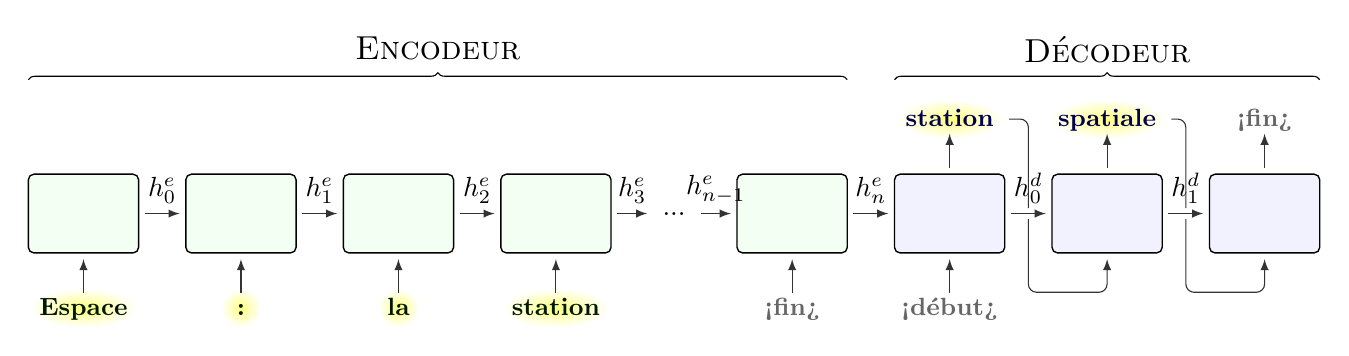
\begin{tikzpicture}

\tikzstyle{cell}=[text centered, rectangle, draw, line width=.5pt, minimum height=1cm, minimum width=1.4cm, rounded corners=2pt]
\tikzstyle{word}=[font=\small\bfseries, text centered, minimum size=.5cm, minimum height=.3cm, text height=1.5ex, text depth=.25ex]
\tikzstyle{vector}=[text centered, rectangle, draw, line width=.5pt, minimum height=.5cm, minimum width=1cm, rounded corners=2pt]
\tikzstyle{arrow}=[shorten >= 2pt, shorten <= 2pt, draw=black!80]

\node[cell, fill=enccolor] (E1) at (0,0){};
\node[cell, fill=enccolor] (E2) at (2,0){};
\node[cell, fill=enccolor] (E3) at (4,0){};
\node[cell, fill=enccolor] (E4) at (6,0){};
\node[text centered] (E5) at (7.5,0){...};
\node[cell, fill=enccolor] (E6) at (9,0){};

\node[word, color=inputcolor, inner color=yellow!50, outer color=white] (I1) at (0,-1.2){Espace};
\node[word, color=inputcolor, inner color=yellow!50, outer color=white] (I2) at (2,-1.2){:};
\node[word, color=inputcolor, inner color=yellow!50, outer color=white] (I3) at (4,-1.2){la};
\node[word, color=inputcolor, inner color=yellow!50, outer color=white] (I4) at (6,-1.2){station};
%\node[word, color=inputcolor, inner color=yellow!50, outer color=white] (I5) at (8,-1.2){...};
\node[word, color=startendcolor] (I6) at (9,-1.2){<fin>};

%\node[cell, fill=veccolor, word, rotate=90] (V) at (11,0){vecteur de pensée};

\node[cell, fill=deccolor] (D1) at (11,0){};
\node[cell, fill=deccolor] (D2) at (13,0){};
\node[cell, fill=deccolor] (D3) at (15,0){};
%\node[cell, fill=deccolor] (D4) at (20,0){};

\node[word, color=startendcolor] (I7) at (11,-1.2){<début>};
\node[word, color=outputcolor, inner color=yellow!50, outer color=white] (O1) at (11,1.2){station};
\node[word, color=outputcolor, inner color=yellow!50, outer color=white] (O2) at (13,1.2){spatiale};
\node[word, color=startendcolor] (O3) at (15,1.2){<fin>};

\draw[->,>=latex,arrow] (E1) -- (E2) node[above,midway] {$h^e_0$};
\draw[->,>=latex,arrow] (E2) -- (E3) node[above,midway] {$h^e_1$};
\draw[->,>=latex,arrow] (E3) -- (E4) node[above,midway] {$h^e_2$};
\draw[->,>=latex,arrow] (E4) -- (E5) node[above,midway] {$h^e_3$};
%\draw[->,>=latex,arrow] (E5) -- (E6) node[above,midway] {$h^e_{n-1}$};
\draw[->,>=latex,arrow] (E5) -- (E6) node[above,midway] {$h^e_{n-1}$};

\draw[->,>=latex,arrow,shorten <= -2pt] (I1) to (E1);
\draw[->,>=latex,arrow,shorten <= -2pt] (I2) to (E2);
\draw[->,>=latex,arrow,shorten <= -2pt] (I3) to (E3);
\draw[->,>=latex,arrow,shorten <= -2pt] (I4) to (E4);
%\draw[->,>=latex,arrow,shorten <= -2pt] (I5) to (E5);
\draw[->,>=latex,arrow,shorten <= -2pt] (I6) to (E6);
\draw[->,>=latex,arrow,shorten <= -2pt] (I7) to (D1);


\draw[->,>=latex, arrow] (E6) -- (D1) node[above,midway] {$h^e_n$};

\draw[->,>=latex,arrow] (D1) -- (D2) node[above,midway] {$h^d_0$};
\draw[->,>=latex,arrow] (D2) -- (D3) node[above,midway] {$h^d_1$};
%\draw[->,>=latex,arrow] (D3) to (D4);

\draw[->,>=latex,arrow,shorten >= -2pt] (D1) to (O1);
\draw[->,>=latex,arrow,shorten >= -2pt] (D2) to (O2);
\draw[->,>=latex,arrow,shorten >= -2pt] (D3) to (O3);
%\draw[->,>=latex,arrow,shorten >= -2pt] (D4) to (O4);

%\node at (5,2) {\large{\textsc{Encodeur}}};
%\node at (17,2) {\large{\textsc{Décodeur}}};

\draw[arrow, rounded corners=3pt] (O1) -| (12, 0);
\draw[->,>=latex, arrow, rounded corners=3pt] (12, 0) -- (12, -1) -| (D2.south);

\draw[arrow, rounded corners=3pt] (O2) -| (14, 0);
\draw[->,>=latex, arrow, rounded corners=3pt] (14, 0) -- (14, -1) -| (D3.south);

%\draw[arrow, rounded corners=3pt] (O3) -| (19, 0);
%\draw[->,>=latex, arrow, rounded corners=3pt] (19, 0) -- (19, -1) -| (D4.south);

\draw[decoration={brace},decorate] (-0.7,1.7) -- node[below=-1.9em] {\large{\textsc{Encodeur}}} (9.7,1.7);
\draw[decoration={brace},decorate] (10.3,1.7) -- node[below=-1.9em] {\large{\textsc{Décodeur}}} (15.7,1.7);


\end{tikzpicture}
}

\caption{Exemple de modèle \textit{encodeur-décodeur} récurrent appliqué à l'extraction automatique de mots-clés.}
\label{fig:seq2seq}
\end{figure}


Le processus d'encodage et de décodage est décrit par l'équation~\ref{eq:enc-dec} et la figure~\ref{fig:seq2seq}.
Dans un premier temps la séquence d'entrée $X$ de taille $n$ est encodée dans le vecteur de pensée $h^e_n$.
Ce vecteur $h^e_n$ est utilisé pour initialiser le premier état caché du décodeur $h^d_0$.
Le décodeur génère ensuite les mots $\hat{y}_t$ qui composent la séquence de sortie $\hat{Y}$ à partir de cet état caché.

\begin{equation}\label{eq:enc-dec}
  \begin{split}
    p(\hat{y}_t | y_{1,...,t-1},h_0) & = \textsc{Softmax}(\sigma(b_v + W_v * h^d_t)) \\
    h^d_t & = \textsc{Rnn}^d(\hat{y}_{t-1}, h^d_{t-1}) \\
    \hat{y}_0 & = \textsc{Debut} \\
    h^d_0 & = h^e_n \\
    h^e_n & = \textsc{Rnn}^e(X) \\
  \end{split}
\end{equation}

Nous présentons ci-après deux améliorations de ce paradigme.
%
D'abord, le mécanisme d'attention qui permet de porter attention à une partie spécifique de l'entrée lors du décodage. Par exemple, la description d'une image nécessite d'identifier les différents objets qui la composent.
%
Ensuite, le mécanisme de copie qui pallie l'incomplétude du vocabulaire de sortie. Ce mécanisme permet au décodeur de copier un mot du document d'entrée au lieu de le générer à partir du vocabulaire de sortie. Le mécanisme de copie est particulièrement utile pour les entités nommées par exemple. Ces entités sont peu fréquentes et ne font généralement pas partie du vocabulaire de sortie.

% Convolution
%Les réseaux de neurones à convolution sont surtout utilisés pour le traitement d'images. Dans le cas du texte, des 
    
% Graphes
%Les réseaux à convolution de graphes (GCN) permettent d'obtenir pour chaque noeud d'un graphe un embedding en fonction de ses voisins. Le nombre de convolutions représente le nombre de bonds qui sont fait entre les noeuds.
    
% Transformer
%Les transformer ont été introduit par \cite{vaswani_attention_2017} et utilisent un mécanisme de self-attention pour chaque mot d'une séquence, de sorte à obtenir pour chaque mot un vecteur qui représente sa relation avec chaque autre mot. Ce mécanisme ne prend pas en compte la séquentialité, en effet chaque calcul est parallélisable. Et ce modèle qui requiert une force de calcul colossale a montré de très bons résultats sur de nombreuse tâches.

\subsubsection{Mécanisme d'attention}
\label{sub:attention_mecanism}

Le mécanisme d'attention~\cite{bahdanau_neural_2014,luong_effective_2015} a été introduit pour améliorer le traitement de longues séquences en permettant au modèle de se focaliser sur certaines parties du document lors du décodage.
%
En effet, un mot-clé concerne seulement certains aspects d'un document. Ce mécanisme permet donc au modèle de porter attention aux parties du document liées à ces aspects.
%
De plus, cette attention au document peut être visualisée grâce aux \emph{poids d'attention} calculés à chaque étape de décodage.
%Par exemple, dans le cadre de la traduction automatique, il permet de visualiser l'alignement entre la phrase en langue source et la phrase en langue cible.
%Par exemple, dans le cadre de la traduction automatique, ce mécanisme permet de visualiser l'importance de chaque mot du document source pour générer la traduction.
La figure~\ref{fig:attention_alignment} illustre cette attention dans le cadre de la traduction automatique pour traduire en français la phrase \say{The agreement on the European Economic Area was signed in August 1992.}
%Il existe généralement un alignement monotone entre les phrases en français et les phrases en anglais.
%Mais ce n'est pas toujours le cas comme le montre le syntagne nominal \say{European Economic Area} dont les mots de la traduction sont dans un ordre inverse \say{zone économique européenne}.
%Le modèle a pu, grâce au mécanisme d'attention, proposer la bonne traduction \say{zone économique européenne} dont l'ordre des mots est inverse à sa traduction.
% Même si le français et l'anglais peuvent généralemnt être traduit mot à mot de manière monotone, le mécanisme d'attention nous permet de visualiser l'alignement non monotone entre zone économique européenne et European Economic Area, en effet l'ordre des noms et adjectifs en français et en anglais est différent.
%Ainsi nous pouvons observer que pour traduire \say{was} en \say{a été}, le modèle à porté attention à \say{was signed} pour comprendre que \say{was} fait parti de la construction du prétérit.
%Pour illustrer ce mécanisme dans le cadre de la traduction automatique nous prenons l'exemple suivant: pour traduire la séquence \say{the European Economic Area} en français (\say{\foreign{la zone économique européenne}}) le modèle portera attention à chaque mot du texte source. Ainsi, pour générer \say{la} et \say{zone} il devra porter attention à \say{\foreign{the}} et \say{\foreign{Area}}. \todo{A revoir.}

\begin{figure}
    \centering
    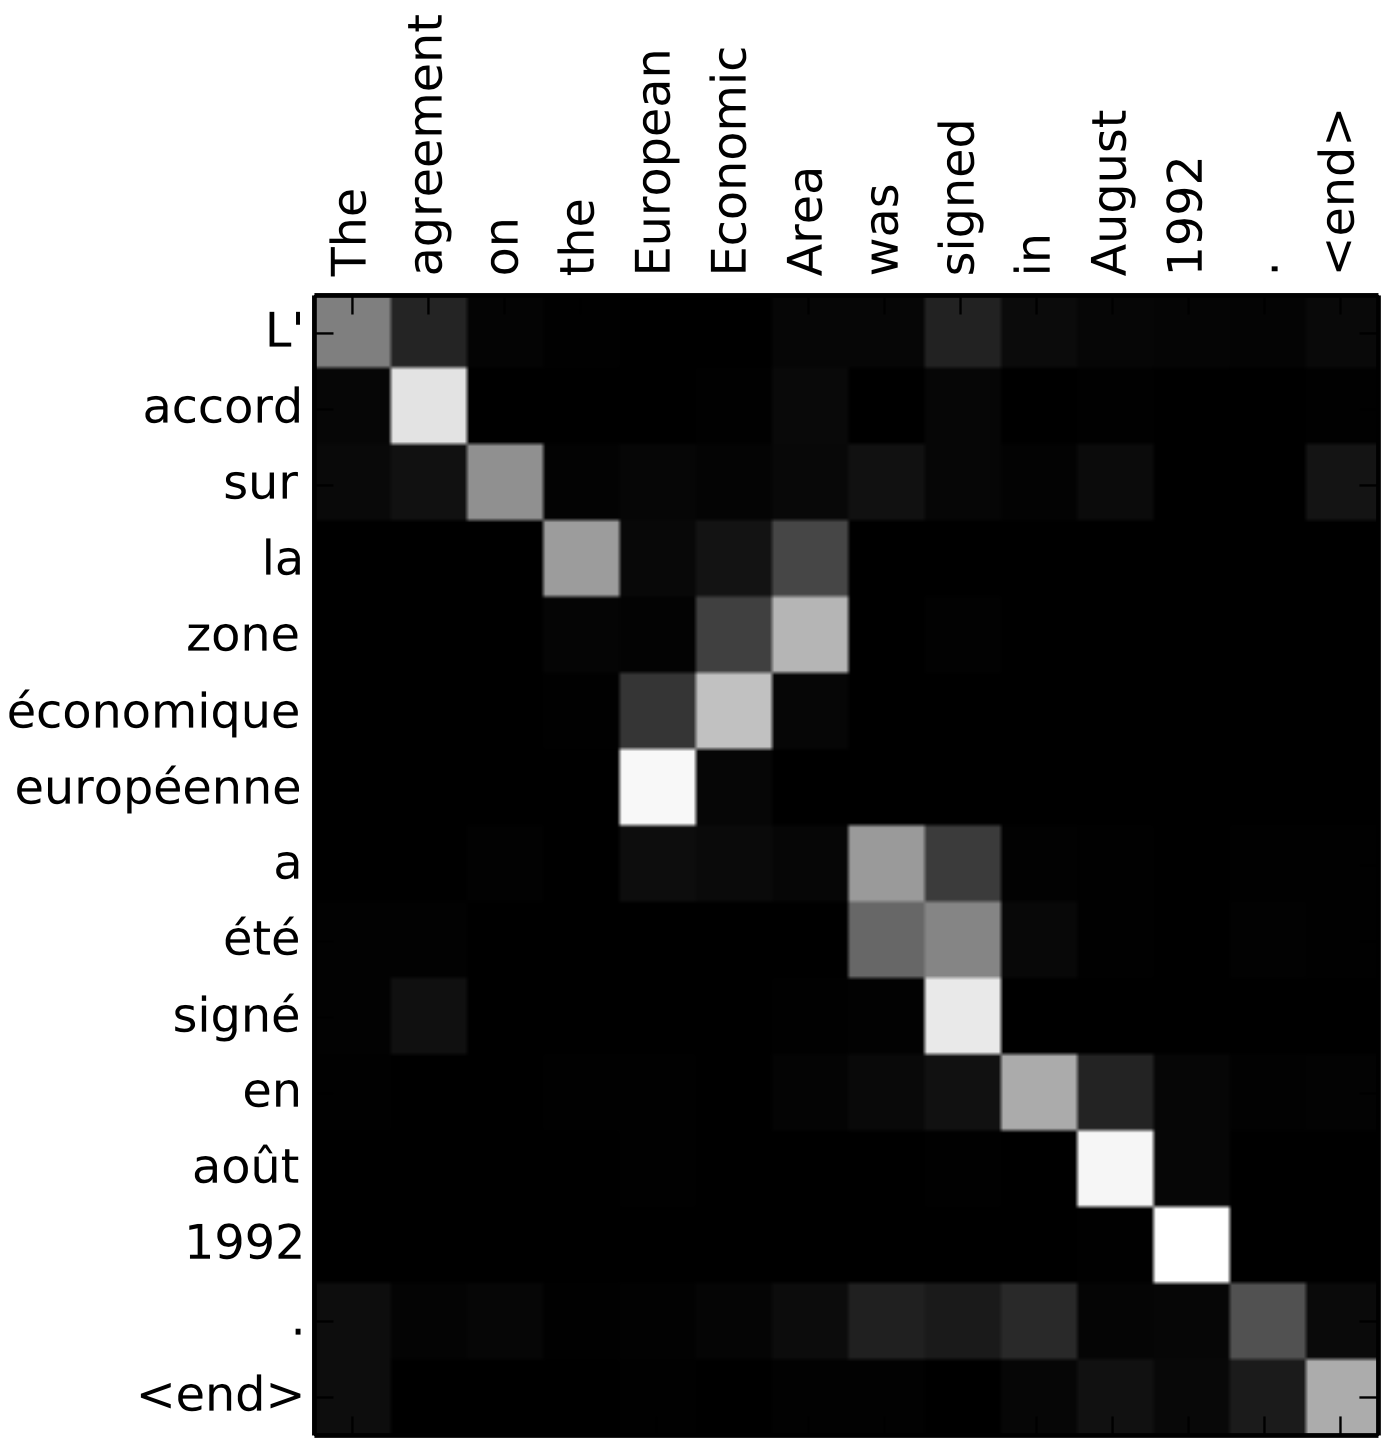
\includegraphics[scale=0.3]{2_production_mots_cles/attention_alignment.png}
    \caption{Exemple de visualisation des poids d'alignement du mécanisme d'attention entre une phrase en anglais et sa traduction en français. Chaque ligne montre la distribution des poids $\alpha_{t}$ ayant servis à générer le mot correspondant en français. Une case blanche indique un poids de 1, une case noire indique un poids de 0. Image extraite de \citet{bahdanau_neural_2014}.}
    \label{fig:attention_alignment}
\end{figure}

%Il faudra aussi porter attention à la syntaxe des deux langues
%Les poids d'attention peuvent être utilisés pour visualiser l'alignement entre les mots de la séquence d'entrée et ceux de la séquence de sortie.
%La figure~\ref{fig:attention_alignment} montre les poids d'alignement dans le cadre de la traduction automatique entre une phrase en anglais et sa traduction en français.

Le décodeur utilise l'état caché courant $h^d_t$ pour générer un mot, le mécanisme d'attention lui permet d'utiliser aussi tous les états cachés de l'encodeur $h^e$ pour mettre à jour l'état caché du décodeur $h^d_t$. Ce mécanisme est décrit dans l'équation~\ref{eq:attention}.
Dans le mécanisme d'attention, les états cachés $h^e$ sont pondérés en fonction de leur importance pour générer le mot $\hat{y}_t$.
Cette importance est établie grâce à une fonction d'alignement $a$ qui calcule une similarité entre l'état caché courant $h^d_t$ et ceux de l'encodeur $h^e$.
Les états cachés $h^e$ sont ainsi moyennés dans le vecteur de contexte $c_t$ utilisé pour mettre à jour l'état caché courant du décodeur $h^d_t$.

Dans l'équation \ref{eq:attention}: $[u;v]$ représente l'opération de concaténation des vecteurs $u$ et $v$; $a$ est une fonction d'alignement qui calcule la similarité entre un état caché de l'encodeur $h^e_t$ et du décodeur $h^d_t$; $\alpha$ représente les poids d'alignement entre les états cachés de l'encodeur $h^e$ et du décodeur $h^d$;  et $\textsc{Softmax}$ est une fonction qui normalise les valeurs d'un vecteur pour qu'il somme à 1.


\iffalse
    \begin{figure}
        \centering
        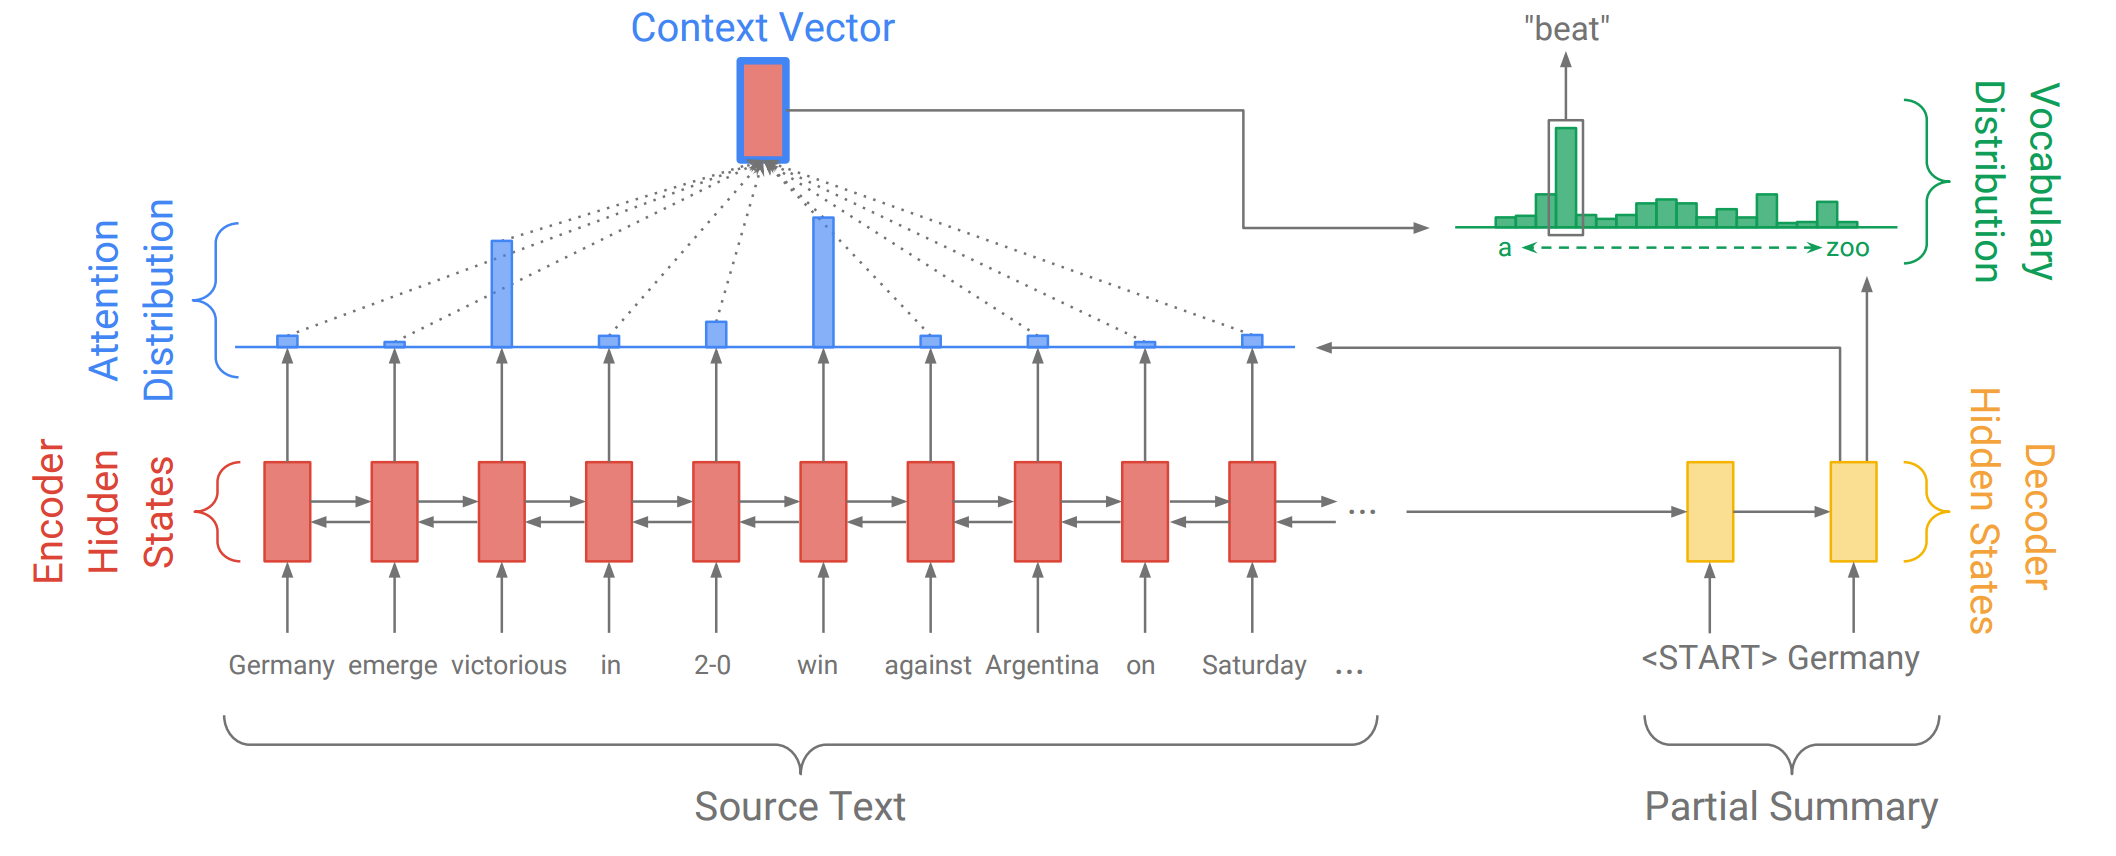
\includegraphics[width=\linewidth]{figures/see_seq2seq-attn.png}
        \caption{Schéma du mécanisme de copie présenté par \cite{see_get_2017}.}
        \label{fig:see_attention}
    \end{figure}
\fi

\begin{equation}\label{eq:attention}
  \begin{split}
    %\hat{Y}_t & = \sigma(b_v + W_v * h^d_t) \\
    p(y_t|y_{<t},x) & = \textsc{Softmax}(\sigma(W_v h^d_t)) \\[.3em]
    h^d_t & = \textsc{Rnn}(y_{t-1}, [h^d_{t-1};c_t]  \\[.3em]
    c_t & = \sum^{|h^e|}_{i=0} \alpha_{i,t} h^e_i \\
    \alpha_{t} & = \textsc{Softmax}(a(h^d_t, h^e)) \\
    %\textsc{Softmax}(x) & = \left[ \frac{x_i}{\sum^{|x|}_{i=0} x_i} , i \in |x| \right]
  \end{split}
\end{equation}

%Le concept d'attention a été présenté de deux manières différentes par \cite{bahdanau_neural_2014} et \cite{luong_effective_2015}.
%
%L'idée de l'attention présentée par~\cite{luong_effective_2015} est \emph{d'utiliser le vecteur de contexte pour prédire $y_t$}.
%
%\cite{bahdanau_neural_2014} présente un autre mécanisme d'attention dont l'idée est de calculer l'état caché du décodeur à l'aide d'un vecteur de contexte. Par rapport à un décodeur classique, seul le calcul de $h^d_t$ change.

\iffalse
    L'idée de l'attention présentée par~\cite{luong_effective_2015} est \emph{d'utiliser le vecteur de contexte pour prédire $y_t$}.
    
    Pour cela, un nouveau $\hat{h}^d_t$ est calculé en fonction d'un vecteur de contexte $c_t$ et de $h^d_t$ (calculé en fonction de $y_{t-1}$ et $h^d_{t-1}$). $c_t$ est la moyenne des $h^e$ pondérés par les scores d'alignement $\alpha$.
    
    Dans leur article, deux manières de calculer l'attention sont présentées: une attention globale et une attention locale.
    %
    Pour l'attention globale, le vecteur de contexte est la moyenne pondérée de toutes les représentations de l'encodeur.
    %
    Pour l'attention locale, le vecteur de contexte est la moyenne pondérée des représentations $h^e$ dans une fenêtre de taille $D$ autour de $h^e_{p_t}$.
    %
    $p_t$ est une valeur entre 0 et $|h^e|$ qui définit le centre de la fenêtre, et peut être calculé de différentes manières.\footnote{Pour plus de détails voir la section 3.2 de \cite{luong_effective_2015}}
    %$p_t$ étant $t$ (dans la traduction automatique on considère que le mot cible $y_t$ est aligné avec le mot source $x_{p_t}$), ou alors un réel entre 0 et $|h^e|$ calculé à l'aide 
    
    \begin{align}
        %y_t & = \sigma(W_v h^d_t) \\
        p(y_t | y_{<t}, x) & = \textsc{Softmax}(W_v \hat{h}^d_t) \\
        \hat{h}^d_t & = \sigma(W_c [c_t;h^d_t]) \\
        c_t & = \sum^{|h^e|}_{i=0} \alpha_{i,t} * h^e_i \\
        \alpha_{i,t} & = \textsc{Softmax}(a(h^e_i, h^d_t)) \\
        h^d_t & = \textsc{Rnn}(y_{t-1}, h^d_{t-1})
    \end{align}
    
    \cite{bahdanau_neural_2014} présente un autre mécanisme d'attention dont l'idée est de calculer l'état caché du décodeur à l'aide d'un vecteur de contexte. Par rapport à un décodeur classique, seul le calcul de $h^d_t$ change. Le calcul du vecteur de contexte est similaire à celui de ~\cite{luong_effective_2015}.
    
    \begin{align}
        p(y_t|y_{<t},x) & = \textsc{Softmax}(W_v h^d_t) \\
        h^d_t & = \textsc{Rnn}(y_{t-1}, [h^d_{t-1};c_t]  \\
        c_t & = \sum^{|h^e|}_{i=0} \alpha_{i,t} * h^e_i \\
        \alpha_{i,t} & = \textsc{Softmax}(a(h^e_i, h^d_t))
    \end{align}
    
    Il existe différentes fonctions d'alignement:
    
    bahdanau $a(h^e_i, h^d_t) = v_a \text{tanh}(W_a h^d_t + U_a h^e_i)$
    
    dot $a(h^e_i, h^d_t) = h^e_i h^d_t$
    
    general $a(h^e_i, h^d_t) = h^e_i W_a h^d_t$
    
    concat $a(h^e_i, h^d_t) = W_a [h^e_i;h^d_t]$
\fi

\subsubsection{Mécanisme de copie}
\label{sub:copy_mecanism}

Le mécanisme de copie~\cite{see_get_2017,gu_incorporating_2016} provient des tâches de traduction automatique et de résumé automatique. Il a pour but de produire des mots peu fréquents ou hors du vocabulaire de sortie.
En effet, les modèles neuronaux qui génèrent du texte choisissent les mots dans un vocabulaire de sortie comportant généralement \num{50 000} mots.
Dans les tâches sus-citées, les mots peu fréquents qui ne font pas partie du vocabulaire de sortie, comme les entités nommées ou les transfuges, doivent pourtant apparaître dans la séquence de sortie.
%Le mécanisme de copie ~\cite{see_get_2017,gu_incorporating_2016} pallie ce problème en permettant au décodeur de générer un mot du vocabulaire de sortie ou bien de copier un mot du document.
Deux mécanismes de copie ont été proposés par \citet{see_get_2017} et \citet{gu_incorporating_2016}; les deux étant similaires, nous présentons ici le premier car plus simple. Il est décrit dans l'équation~\ref{eq:copy_mecanism}.

% exemple
%Le mécanisme d'attention a été utilisé comme post-traitement pour remplacer les mots inconnus de la sortie par les mots de l'entrée alignés par le mécanisme d'attention. Ceci permettant de traiter les entités nommées peu fréquentes ou les transfuges.
%
%Le mécanisme de copie vient automatiser ce processus en permettant au modèle de générer un mot du vocabulaire ou de copier un mot du document.

%, tous deux inspirés des réseaux de pointeurs~\cite{vinyals_pointer_2015} qui génèrent une séquence de pointeurs vers la séquence d'entrée.
Ce mécanisme utilise le vocabulaire de la séquence d'entrée $\mathcal{X}$ (particulier à chaque document) en plus du vocabulaire de sortie $\mathcal{V}$.
Pour produire un mot, une distribution de probabilité sur le vocabulaire  $P_{vocab}(y_{t})$ est calculée comme précédemment par le décodeur (cf. section~\ref{sub:decoding}) et les poids du mécanisme d'attention $\alpha$ (cf. section~\ref{sub:attention_mecanism}) sont utilisés pour estimer la probabilité de copie de chaque mot du document.
Les poids d'attention $\alpha$ des mots qui apparaissent plusieurs fois dans l'entrée $x$ sont sommés $\sum_{j,x_j=y_{t,i}} \alpha^t_j$.
Ainsi, un mot peut être généré à partir du vocabulaire de sortie $\mathcal{V}$ ou copié à partir du vocabulaire du document $\mathcal{X}$.
Les probabilités de copie et de génération d'un même mot, qui appartient au document et au vocabulaire, sont sommées.
Dans l'équation~\ref{eq:copy_mecanism}: $h^d_t$, $c_t$ et $\alpha^t_j$ proviennent du mécanisme d'attention (cf. équation~\ref{eq:attention}); $p_{gen}$ est un curseur permettant au modèle de privilégier la copie ou la génération et $P_{vocab}(y_t)$ est une distribution de probabilité sur le vocabulaire de sortie $\mathcal{V}$.

%Les probabilités de génération et de copie sont combinés pour donner une distribution de probabilités sur $\mathcal{X} \cup \mathcal{V}$.

\begin{equation}\label{eq:copy_mecanism}
  \begin{split}
    p(y_{t,i}|y_{<t},x) & = p_{gen} P_{vocab}(y_{t,i}) + (1 - p_{gen}) \sum_{j,x_j=y_{t,i}} \alpha^t_j \\
    p_{gen} & = \sigma(W_h h^d_t + W_c c_t + W_y y_{t-1}) \\
    P_{vocab}(y_{t}) & = \textsc{Softmax}(\sigma(W_v h^d_t))
  \end{split}
\end{equation}

%ou les poids d'un mécanisme d'attention supplémentaire, utilisé seulement pour calculer le score de copie, pour~\cite{gu_incorporating_2016}

\iffalse
    %\cite{gu_incorporating_2016}, création d'un vocabulaire spécifique a chaque instance, composé de $\mathcal{V}$ le vocabulaire normal et $\mathcal{X}$ le vocabulaire des mots de l'entrée.
    %
    %Ça change le calcul de $y_t$ par rapport au mécanisme d'attention.
    %
    %On défini les vecteurs $\psi_g \in \mathds{R}^|\mathcal{V}|$ et $\psi_c \in \mathds{R}^|\mathcal{X}|$ qui contiennent respectivement les score de copie et de génération.
    
    % attentive read = les poids de l'attention
    % selective read = les poids de l'"attention" du mécanisme de copie
    
    \begin{align}
        y_t & = \textsc{Softmax}(e^{P_{gen}} +e^{P_{copy}}) \\
        P_{gen} & = W_v h^d_t \\
        P_{copy} & = \left[ \sum^{|h^e|}_{j=0, x_j=x_i} \sigma(h^e_j W_c) h^d_t | x_i \in \mathcal{X} \right] \\
        h^d_t & = RNN([y_{t-1};cc_t)],h^d_{t-1}) \\
        cc_t & = \sum^{|h^e|}_{i=1} aa_{t,i} h^e_t \\
        aa_{t,i} & = \textsc{Softmax}()
    \end{align}
    
    %\cite{see_get_2017} reprend le mécanisme d'attention de \cite{luong_effective_2015} et modifie le calcul de $y_t$ en ajoutant une probabilité de copie et un curseur privilégiant la copie ou la génération.
    
    \begin{align}
        p(y_{t,i}) = p_{gen} P_{vocab}(y_{t,i}) + (1 - p_{gen}) \sum_{j,x_j=y_{t,i}} \alpha^t_j \\
        p_{gen} = \sigma(W_c c_t + W_h h^d_t + W_y y_{t-1})
    \end{align}
\fi

% Multitache
% Conditional Random Field
% Reinforcement Learning : adaptative reward


\section{Méthodes de bout-en-bout}
\label{methodes-de-bout-en-bout}

\todo{Ajouter des schéma pour mieux comprendre les méthodes.}

Dans cette section nous présentons un état de l'art des méthodes de bout-en-bout.
Ces méthodes, contrairement aux méthodes en chaîne de traitement (cf. section~\ref{sec:methode-en-chaine-de-traitement}), prennent en entrée un document et laissent le soin au modèle d'en extraire les caractéristiques pour retourner un ensemble de mots-clés sans étapes intermédiaires ni définition manuelle de ces caractéristiques.
Parmi les méthodes proposées dans la littérature, nous distinguons les méthodes génératives, qui peuvent produire des mots-clés présents et des mots-clés absents, des méthodes extractives, limitées aux mots-clés présents.

Jusqu'à présent, toutes les méthodes de bout-en-bout qui ont été proposées sont supervisées et reposent sur des réseaux de neurones (cf. section~\ref{sub:neural_network}) qui nécessitent de grandes quantités de données annotées pour être entraînées.
%
Le développement de ces méthodes démarre avec l'introduction du jeu de données KP20k et de la méthode générative CopyRNN par \citet{meng_deep_2017}.
Le jeu de données KP20k, qui comporte $\simeq$\num{550000} documents, comble un manque.
En effet, seuls de petits jeux de données (de l'ordre du millier de documents) étaient jusqu'alors disponibles.
Ce travail a ainsi lancé une nouvelle direction de recherche sur les méthodes génératives de production de mot-clés.

\begin{figure}
    \centering
    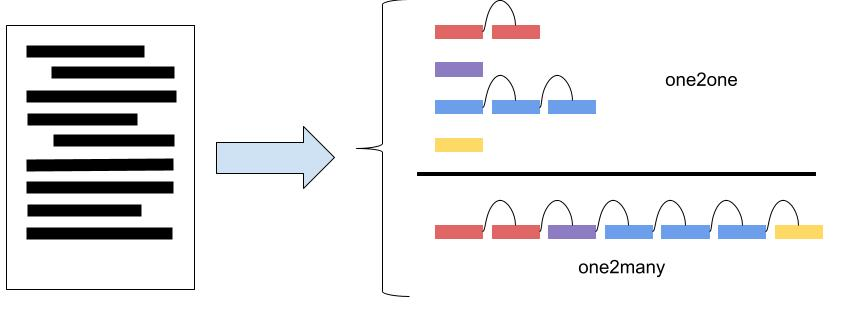
\includegraphics[scale=0.4]{2_production_mots_cles/Decoding strategies.jpg}
    \caption{Représentation schématique des stratégies de décodage \emph{one2one} et \emph{one2many}.}
    \label{fig:decoding_strategies}
\end{figure}
\todo{Refaire en tikz}

Dans cet état de l'art, nous présentons tout d'abord les méthodes automatiques de génération de mots-clés de bout-en-bout, qui sont au c\oe{}ur de ce travail de thèse.
Nous présentons ces méthodes de génération en deux parties: premièrement, les méthodes qui générent les mots-clés un à un (\emph{one2one}), et deuxièmement, celles qui génèrent des séquences de mots-clés (\emph{one2many}). Ces deux types de génération sont schématisés dans la figure~\ref{fig:decoding_strategies}.
Nous présentons ensuite les méthodes extractives de bout-en-bout, c'est-à-dire celles qui se limitent aux seuls mots-clés présents.

\subsection{Génération de mots-clés}
\label{sub:generation_de_mots_cles}

Les méthodes génératives, introduites par \citet{meng_deep_2017}, ont pour objectif de pallier deux faiblesses qui concernent la majorité des méthodes extractives présentées précédemment: l'impossibilité de produire des mots-clés absents ainsi que la faible prise en compte de la sémantique.
Le paradigme encodeur-décodeur sur lequel les méthodes génératives sont fondées permet d'encoder la sémantique du document.
Ainsi, les mots-clés produits sont le fruit d'une \say{compréhension} du document, contrairement aux méthodes en chaîne de traitement qui s'intéressent à l'\say{importance} des mots dans le document indépendamment de leur sens.
%
Ces méthodes génératives rendent possible la production de mots-clés absents grâce à la manière dont le décodeur génère la séquence de sortie.
Ce processus s'effectue en choisissant, à chaque étape de décodage, un mot à partir d'un vocabulaire de sortie qui est plus grand et différent du vocabulaire du document.
Ces méthodes génératives apprennent à générer des mots-clés un par un (génération \emph{one2one}, voir figure~\ref{fig:decoding_strategies}), c'est-à-dire que chaque document $X$ et son ensemble de mot-clés $Y$ de taille $N$ forment un couple $(X, \{Y_0, ..., Y_N\})$, décomposé en autant d'exemples d'entraînement que de mots-clés, $(X, Y_0), ... , (X, Y_N)$.

%\paragraph{Définitions}
%\todo{Il faudrait définir avant les principaux modèles: one2one, séquence avant de les définir formellement; Fait ausi des dessins}
%$x$ et $y$ représentent des mots, $p$ des mots-clés. Étant donné un ensemble de données $D = {(x^i,p^i), i \in 1...N}$ de taille $N$, un exemple est composé d'un document $x^i$ et d'un ensemble de mots-clés $p^i = {p^i_j, j \in 1...M^i}$ de taille $M^i$. Les documents et les mots-clés sont composés de mots $[x^i_k, k \in 1...N^i]$ et $[y^i_j]$ est composé d'un document composé d'une séquence de mots $x^i = (x^i_1, ..., x^i_{N^i})$ de longueur $N^i$ et d'un ensemble de mots-clés $p^i$ de taille $M^i$ avec $p^i = (p^i_1, ..., p^i_{M^i})$, où chaque mot-clé est une séquence de mots de taille $M^{i,j}$ avec $p^{i,j} = (y^{i,j}_1, ..., y^{i,j}_{M^{i,j}})$. Dans le cadre des modèles one2one, un couple document -- mots-clés est découpé en $M^i$ différents couples $(x^i, p^{i,1}), ..., (x^i, p^{i, M^i})$. 
%Pour les modèles en séquences, les mots-clés sont concaténés de sorte à former une unique séquence $(x^i, y^{i,1}_1 \lozenge ... \lozenge y^{i,1}_{M^{i,j}} \lozenge \text{SEP} \lozenge y^{i,2}_1 \lozenge ... \lozenge y^{i,M^i}_{M^{i,j}})$.

La méthode pionnière de génération automatique de mots-clés appliquée aux documents scientifiques est CopyRNN~\cite{meng_deep_2017}.
%
L'architecture neuronale de cette méthode s'inspire du processus d'annotation humain qui consiste à lire le document pour le comprendre dans son entièreté puis à le résumer grâce à des mots-clés.
%Aussi, les humains peuvent facilement s'abstraire du texte et faire appel à leurs connaissances pour produire des mots-clés qui n'apparaissent pas dans le texte.
Pour reproduire ce processus, CopyRNN utilise le paradigme encodeur-décodeur, que nous avons présenté dans la section~\ref{sub:paradigme_encodeur_decodeur}, pour encoder un document et le décoder ensuite en un mot-clé. % Ainsi un réseau de neurones récurrent encode le document dans un vecteur de pensée, puis un autre décode, génère, ce vecteur de pensée en un mot-clé.
Pour améliorer les performances des modèles encodeur-décodeur, il est commun d'utiliser un mécanisme d'attention (voir section~\ref{sub:attention_mecanism}).
Ce mécanisme permet au modèle de porter attention à certaines parties du document lors de la génération d'un mot.
%
Un mécanisme de copie est aussi ajouté au modèle pour lui permettre de générer des mots peu fréquents (voir section~\ref{sub:copy_mecanism}).
Ce mécanisme de copie modifie le décodage en permettant de générer un mot à partir du vocabulaire de sortie ou bien à partir du document.\\
%
Cette méthode obtient des performances bien plus élevées que les précédentes méthodes extractives. Les performances de CopyRNN sont de l'ordre de 30 points de \fmesure{} pour les mots-clés présents tandis que les performances des méthodes extractives sont généralement en dessous de 20 points de \fmesure{}.
Les mots-clés absents, qui ne pouvaient jusque-là pas être produits, correspondent peu à la référence: parmi les 50 meilleurs mots-clés absents un seul apparaît dans la référence.


%La communauté scientifique présente de nouvelles méthodes basées sur CopyRNN et tente de l'améliorer.
% les méthodes essaient de résoudre les problèmes identifiés
%Les méthodes présentées augmentent toujours les performances de génération des mots-clés présents et absents.

Certaines méthodes proposées essaient d'améliorer l'encodage du document.
\citet{chen_title-guided_2019}, par exemple, constate que les mots-clés ne sont pas uniformément distribués dans les documents.
En particulier \npercent{60} des mots-clés de référence ont au moins un mot en commun avec le titre du document.
Pour prendre cela en compte, ils proposent TGNet (Title Guided Network), qui étend CopyRNN en introduisant un nouvel encodeur spécifique au titre, en plus de l'encodeur du document.
Cet encodage du titre permet de donner un poids supplémentaire à l'information qu'il contient.
Ces deux représentations (du titre et du document) sont ensuite combinées puis fournies au décodeur.
Cette méthode améliore nettement les performances de génération des mots-clés présents et absents par rapport à CopyRNN (+\npercent{5} sur KP20k).
% Ils ne regardent que la F-mesure présent/absent rien d'autre

La redondance dans les ensembles de mots-clés produits est un problème récurrent dans les méthodes de production de mots-clés.
En effet, \citet{hasan_automatic_2014} montrent que 8 à \npercent{12} des erreurs des méthodes sont liées à la redondance des mots-clés.
Ainsi, les méthodes en chaîne de traitement mettent en place des stratégies, notamment lors de la sélection du sous-ensemble de mots-clés, pour limiter cette redondance (voir section~\ref{choisir-le-sous-ensemble}).
Dans cette ligne de recherche, \citet{zhao_incorporating_2019} remarquent les méthodes de bout-en-bout ne sont pas exemptes de ce problème, ils s'intéressent ainsi au chevauchement entre les mots-clés générés et ceux de référence.
Par exemple, \npercent{23.98} des mots-clés unigrammes générés par CopyRNN font partie d'un mot-clé de référence, et \npercent{47.15} des mots-clés 4-grammes générés par CopyRNN contiennent un mot-clé de référence.
Dans l'optique de limiter ces chevauchement, ils présentent le modèle ParaNet$_T$+CoAtt qui entraîne le modèle, à générer à la fois les mots-clés et leurs étiquettes morphosyntaxiques, ainsi la syntaxe des mots-clés générés sera similaire à celle des mots-clés de référence.
Pour cela ils ajoutent au modèle CopyRNN un encodeur, pour les étiquettes morphosyntaxiques des mots du document, ainsi qu'un décodeur, pour celles du mot-clé.\footnote{Les étiquettes morphosyntaxiques du document et des mots-clés proviennent de l'outils Stanford CoreNLP.}
Les informations des deux décodeurs sont ensuite combinées et utilisées pour générer les mots-clés et leurs étiquettes morphosyntaxiques.
%Grâce à cette méthode, les mots-clés générés chevauchent moins les mots-clés de référence; par exemple le pourcentage de mot-clés 4-grammes contenant un mot-clé de référence a baissé de \npercent{10}.

\begin{figure}
    \centering
    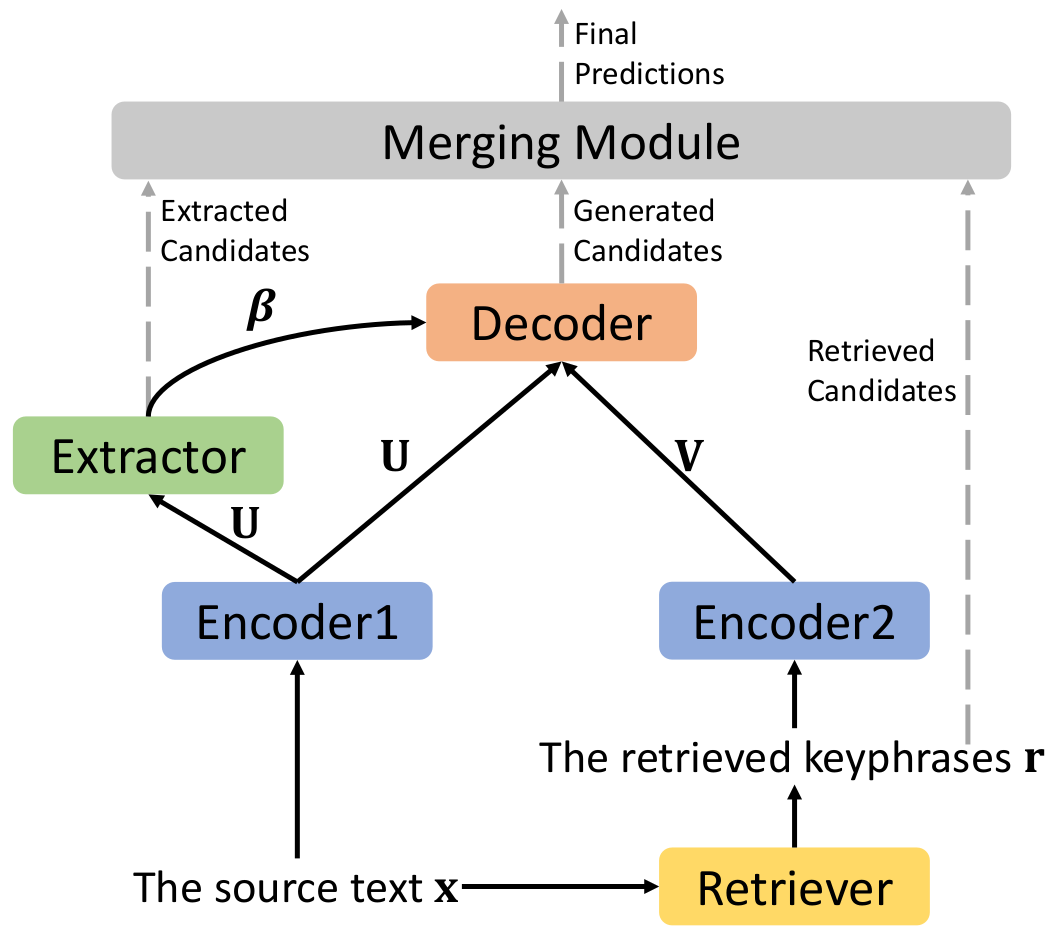
\includegraphics[scale=0.2]{2_production_mots_cles/kg_ke_kr_m.png}
    \caption{Représentation schématique de l'architecture de la méthode KG-KE-KR-M. Image extraite de~\citet{chen_integrated_2019}.}
    \label{fig:schema_kgkekrm}
\end{figure}

%Le processus manuel d'annotation en mots-clés est composé de plusieurs étapes: la lecture du document, l'extraction des mots-clés dans le document puis l'attribution de mots-clés absents du document et enfin la combinaison des mots-clés provenant de ces deux processus d'annotation.
Dans l'optique de reproduire l'annotation humaine, \citet{chen_integrated_2019} propose la méthode KG-KE-KR-M qui produit un ensemble de mots-clés en combinant différentes méthodes: génération de mots-clés, extraction de mots-clés, récupération de mots-clés (voir figure~\ref{fig:schema_kgkekrm}).
%Ces différentes méthodes sont entraînées de bout-en-bout puis les mots-clés de chaque méthode sont pondérés grâce à un classifieur.
%
Dans un premier temps, cette méthode récupère les mots-clés de référence des $K$ documents d'entraînement les plus proches du document traité (grâce à la distance de Jaccard).
Ces mots-clés \emph{récupérés} sont concaténés puis encodés. Ils serviront à conditionner la génération de mots-clés.
Dans un second temps, des mots-clés sont \emph{extraits} du document en classifiant chaque mot comme mot-clé ou non mot-clé.
%Cette classification s'effectue grâce aux états cachés du document encodé.
Ensuite, des mots-clés sont \emph{générés} à partir du document ainsi que des mots-clés récupérés et des mots-clés extraits.
Enfin, les mots-clés récupérés, extraits et générés sont pondérés grâce à un classifieur.
Cette méthode à la particularité de combiner les méthodes en chaîne de traitement (sélection de candidats puis pondération) et les méthodes de bout-en-bout (apprentissage conjoint de la génération et de l'extraction).
Malgré la grande diversité dans les techniques de production de mots-clés candidats, les performances ne sont pas significativement supérieures à CopyRNN. Cette méthode produit néanmoins plus de mots-clés absents de référence que CopyRNN.

La méthode CorrRNN~\cite{chen_keyphrase_2018} considère que les mots-clés doivent couvrir l'ensemble des sujets du document et être divers, c'est-à-dire que chaque mot-clé doit concerner un sujet différent.
Cette méthode étend CopyRNN en y ajoutant un mécanisme de couverture et un mécanisme de revue.
Le mécanisme de couverture encourage le modèle à porter attention aux différentes parties du document.
Il conserve et accumule les scores d'attention des mots du document à chaque étape de décodage, et il est inclus dans le calcul du mécanisme d'attention.
Ensuite, le mécanisme de revue est essentiellement un mécanisme d'attention sur les mots générés.
Son objectif est d'identifier les sujets déjà couverts par les mots-clés générés et ainsi de générer des mots-clés qui concernent des sujets non traités.
Cette méthode est la première à prendre en compte les mots-clés déjà générés dans le processus de génération, pour cela la phase d'entraînement est modifiée.
Au lieu de rétro-propager le gradient après chaque mot-clé de référence, la phase de rétro-propagation n'est effectuée qu'une fois tous les mots-clés de référence du document traités.
%Chaque mot-clé est généré en utilisant les mécanismes de couverture et de redondance, qui prennent en compte les mots-clés déjà générés; le gradient est ensuite calculé grâce à l'erreur de chaque mot-clé; et enfin, rétro-propagé.
%Cette méthode améliore les performance de production de mots-clés présent par rapport à CopyRNN, mais l'article ne présentant pas ses résultats sur le jeu de données de référence KP20k et utilisant des métriques peu utilisés dans les autres travaux la comparaison est limitée.

\subsection{Génération de séquences de mots-clés}% (\textsc{One2Seq})}
%\subsection{Génération en séquence}
\label{sub:generation_de_sequences_de_mots_cles}

%Nous avons présenté dans la section précédente, des méthodes génératives qui apprennent à générer un mot-clé par document.
Nous présentons dans cette section des méthodes qui apprennent à générer des séquences de mots-clés (génération \emph{one2many}, voir figure~\ref{fig:decoding_strategies}). C'est-à-dire que chaque exemple d'entraînement est composé d'un document et de la concaténation des mots-clés de référence en une unique séquence dans laquelle ils sont séparés par un symbole de séparation. Par exemple, l'ensemble de mots-clés $\{$ Classe , Fichier log , Agrégat $\}$ sera transformé en \say{Classe \texttt{SEP} Fichier log \texttt{SEP} Agrégat \texttt{FIN}}.
%Le développement des méthodes utilisant la génération \emph{one2many} part du constat que la génération \emph{one2one} ne permet pas de prendre en compte les mots-clés déjà générés et que les ensembles de mots-clés sont souvent redondants~\cite{hasan_automatic_2014}.
Le développement des méthodes génératives \emph{one2many} part du constat que les ensembles de mots-clés produits sont souvent redondants~\cite{hasan_automatic_2014} et que la génération \emph{one2one} ne permet pas de pallier ce problème.
En effet, les méthodes \emph{one2many} font l'hypothèse qu'avec la génération en séquence, le modèle ayant accès aux mots-clés déjà générés, il ne générera pas de mots-clés redondants.
%
Cette méthode de génération permet au modèle de générer le même nombre de mots-clés que la référence, en effet, il apprend en même temps qu'à générer les mots-clés, à placer les séparateurs de mots-clés et le symbole de fin.
Ainsi, ces méthodes peuvent générer des mots-clés selon deux stratégies~\cite{yuan_one_2020}: l'\textbf{inférence exhaustive} qui utilise l'algorithme de recherche en faisceau pour sur-générer des mots-clés et ainsi en obtenir un nombre fixe pour chaque document, c'est la stratégie employée par les méthodes génératives \emph{one2one}; et l'\textbf{inférence auto-régulée} (\foreign{self-terminating}) dans laquelle le décodage s'arrête lors de la génération du symbole de fin, cette stratégie permet au modèle de produire un nombre pertinent de mots-clés pour le document.
La seconde stratégie de décodage permet donc de s'affranchir du choix arbitraire du nombre de mots-clés $n$ à produire (voir section~\ref{choisir-le-sous-ensemble}).

Pour entraîner ces modèles, les mots-clés sont concaténés, mais ce processus n'est pas trivial.
En effet, l'ordre dans lequel les mots-clés sont concaténés influence les performances des modèles.
L'étude de \citet{meng_empirical_2021} compare différentes manières d'ordonner les mots-clés, telles que: \emph{No-Sort} qui laisse l'ordre par défaut; \emph{Alpha} qui trie par ordre alphabétique; \emph{Pres-Abs} qui place les mots-clés présents avant les mots-clés absents. L'étude montre que c'est l'ordre \emph{Pres-Abs} qui donne les meilleures performances.

La première méthode à générer des séquences de mots-clés est catSeqD~\cite{yuan_one_2020,yuan_generating_2018}.
L'objectif de cette méthode, similaire à CorrRNN, est d'augmenter la diversité des mots-clés générés.
%
Pour cela, le modèle CopyRNN, utilisé comme base, est augmenté d'un mécanisme de couverture sémantique et de régularisation orthogonale pour former le modèle catSeqD.
%
Le mécanisme de \emph{couverture sémantique} repose sur l'hypothèse que l'ensemble de mots-clés de référence et le document encodent la même information.
Ainsi, un nouvel encodeur est entraîné à encoder les mots-clés et à produire la même représentation que pour le document.
Il encode la séquence au fur et à mesure de sa génération et l'état cachés qui en résulte conditionne la prédiction du mot suivant, cela contraint les mots-clés générés à être proche sémantiquement du document.
%
Ensuite, les auteurs constatent que les mots générés après les séparateurs de mots-clés sont souvent similaires.
Le mécanisme de \emph{régularisation orthogonale} pallie ce problème en diversifiant explicitement les représentations des séparateurs, en pénalisant, dans la fonction de coût, ces représentations si elles ne sont pas orthogonales.

\todo{Refaire en Tikz}
\begin{figure}
    \centering
    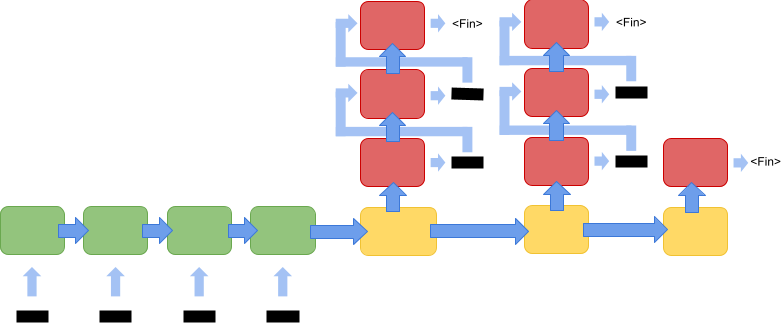
\includegraphics[scale=0.5]{2_production_mots_cles/exhird.png}
    \caption{Représentation schématique du décodage hiérarchique de la méthode ExHirD. L'encodeur du document est représenté en vert, le décodeur de concept en jaune et le décodeur de mots-clés en rouge.}
    \label{fig:schema_exhird}
\end{figure}

Dans le but de mieux modéliser les ensembles de mots-clés, \citet{chen_exclusive_2020} s'intéressent à la structure hiérarchique des ensembles de mots-clés.
En effet, les méthodes de génération de séquences de mots-clés identifient les mots-clés grâce à des marqueurs générés par le modèle. Cette séquentialité ne permet pas de représenter la hiérarchie entre les mots-clés et les mots qui les composent.
Ces travaux se rapprochent de \citet{yuan_generating_2018} qui essaient de rompre la séquentialité en modifiant la représentation des séparateurs de mots-clés avec le mécanisme de régularisation orthogonale.
Ainsi, ils présentent la méthode ExHirD~\cite{chen_exclusive_2020} dans laquelle le décodeur de l'architecture de CopyRNN est remplacé par un décodeur hiérarchique (voir figure~\ref{fig:schema_exhird}) qui génère les mots-clés en deux temps: d'abord l'identification des concepts, ensuite la génération de leur représentation textuelle.
Ce décodeur hiérarchique comprend un premier décodeur qui produit une représentation dense d'un concept, puis un second décodeur qui va générer une séquence de mots à partir de cette représentation dense pour instancier le concept en un mot-clé.
La génération des mots utilise deux mécanismes d'attention sur les documents d'entrée: l'un est conditionné par la représentation dense du concept; l'autre, standard, est conditionné par le mot précédent.
Ainsi, ce décodeur hiérarchique permet de modéliser explicitement les concepts importants du document et les mots qui les décrivent.
%
L'évaluation de cette méthode montre néanmoins un faible gain de performance, de l'ordre d'un point de F@5, pour les mots-clés présents et absents.
%
Ces travaux s'attellent aussi au problème de redondance des mots-clés et proposent un mécanisme de décodage exclusif pour tenter de le résoudre.
Ce mécanisme, simple dans son idée, interdit au modèle de générer deux mots-clés commençant par le même mot.
En effet, les mots-clés comportent le plus souvent entre 1 et 4 mots (voir section~\ref{sub:nature_linguistique}), ainsi le premier mot affecte grandement les suivants.
Ce mécanisme n'est pas limité à la méthode ExHirD; il peut être adapté aux différents types de décodage ou être utilisé en post-traitement.
Son évaluation montre qu'il fait significativement baisser le nombre de mots-clés dupliqués sans faire baisser les scores de F@5.

Les méthodes génératives \emph{one2many} apprennent à déterminer le nombre de mots-clés à produire mais en génèrent trop peu: catSeqD génère en moyenne 4,3 mots-clés par document alors que la référence en est composée de 5,3 en moyenne.
Les travaux de \citet{chan_neural_2019} s'intéressent à encourager les modèles à générer plus de mots-clés, en les entraînant à optimiser le rappel et la \fmesure{}.
Or ces métriques ne peuvent être utilisées comme fonction de coût dans l'algorithme de descente de gradient, car elles ne sont pas dérivables.
Pour résoudre ce problème, les auteurs proposent d'utiliser l'apprentissage par renforcement pour affiner\footnote{\foreign{To fine-tune} en anglais.} des modèles déjà entraînés.
%
Dans l'apprentissage par renforcement~\cite{williams_simple_1992}, un agent produit une série d'actions en suivant une politique (ici la génération de mots grâce à un modèle génératif), puis est récompensé pour chacune des actions.
%Dans l'apprentissage par renforcement~\cite{williams_simple_1992}, un agent produit une série d'actions en suivant une politique puis il est récompensé pour chaque action.
%Dans notre cas, une action consiste à générer un mot, la politique permettant de choisir le mot est un modèle génératif, et la récompense est le rappel ou la f-mesure.
L'algorithme d'apprentissage par renforcement optimise ainsi les poids du modèle (met à jour la politique) en fonction de la récompense.
%
Dans la méthode proposée, la récompense s'adapte selon le nombre de mots-clés générés: s'il est trop faible, la récompense sera le rappel pour encourager le modèle à générer plus de mots-clés; à l'inverse s'il est trop grand, la récompense sera la \fmesure{}, pour encourager le modèle à générer seulement de bons mots-clés.
%
De plus, les mots-clés présents et absents sont récompensés séparément pour favoriser la génération des mots-clés absents.

%CDKGen~\cite{diao_keyphrase_2020} (use close docs to encode, transformers)
%SenseNet~\cite{luo_sensenet_2020} (??)

Les travaux, concernant les méthodes neuronales, présentés jusqu'à présent considèrent que la quantité de données disponibles est suffisante.
Nous verrons dans le chapitre~\ref{chap:framework} que les sources de données contenant des documents annotés en mots-clés sont peu nombreuses malgré la large disponibilité de documents scientifiques en ligne.
Ainsi, les travaux de \citet{ye_semi-supervised_2018} se placent dans un cadre où la quantité de documents annotés est limitée.
%
Pour cela, les auteurs proposent deux méthodes qui tirent parti de la masse de documents non annotés pour la génération de mots-clés.
%
La première méthode consiste à utiliser des documents non annotés en mots-clés dans le cadre d'apprentissage multitâche.
Un réseau de neurones encodeur-décodeur est entraîné, pour les documents annotés, à générer des séquences de mots-clés et, pour les documents non annotés, à générer le titre du document. Dans le modèle, deux décodeurs différents sont utilisés pour chacune des tâches mais l'encodeur est partagé.
%
La seconde méthode consiste à créer un corpus synthétique en annotant automatiquement des documents en mots-clés. Les mots-clés sont extraits grâce aux méthodes \tfidf{} et TextRank.
Ainsi, un modèle de génération de mots-clés est pré-entraîné grâce à la combinaison des corpus synthétique et annoté, puis affiné grâce au seul corpus annoté.
%
L'évaluation des deux modèles résultant de ces méthodes d'entraînement montre qu'ils obtiennent des résultats similaires.
Les scores de F@5 pour les mots-clés présents des modèles semi-supervisés sont comparables à ceux du modèle \emph{catSeq} (CopyRNN entraîné à générer des séquences de mots-clés), bien qu'ils n'utilisent qu'un dixième des documents annotés utilisés par \emph{catSeq}.

\subsection{Extraction de mots-clés}

% Chapeau
Les méthodes génératives de bout-en-bout sont très performantes pour produire des mots-clés présents, mais génèrent très peu de mots-clés absents.
Ainsi, la communauté scientifique s'intéresse à des méthodes de bout-en-bout exclusivement extractives.
%Les méthodes génératives de bout-en-bout sont très performantes pour produire des mots-clés présents, ainsi la communauté scientifique s'intéresse à 
%Les méthodes génératives de bout-en-bout, qui ont la particularité de produire des mots-clés absents, n'en produisent au final que très peu~\cite[inter alia]{chen_exclusive_2020, santosh_hicova_2021} et ceux-ci ne correspondent que très peu aux mots-clés de référence~\cite[inter alia]{ahmad_select_2020, ye_one2set_2021}.
%Mais leurs performances élevées pour produire des mots-clés présents encouragent tout de même le développement de méthodes de bout-en-bout.
%C'est pourquoi la communauté scientifique s'intéresse aux méthodes de bout-en-bout exclusivement extractives.
%
Bien qu'elles ne soient pas au c\oe{}ur de nos travaux, nous présentons les principales méthodes extractives par soucis d'exhaustivité.
% Plan
Dans cette section nous présentons tout d'abord les méthodes fondées sur l'annotation en séquence, ensuite, une méthode de classification, et enfin, une méthode fondée sur les graphes.

Le développement de ces méthodes est lié à celui des modèles de langues pré-entraînés tels que BERT~\cite{devlin_bert_2019}, SciBERT~\cite{beltagy_scibert_2019} ou encore GPT-2~\cite{radford_language_2019} qui reposent sur l'architecture transformer~\cite{vaswani_attention_2017}.
Ils sont utilisés pour fournir des plongements de mots contextuels ou bien pour être affinés pour une tâche particulière.
Ces modèles, entraînés sur de très grandes quantités de données, ont permis d'améliorer significativement les performances de nombreuses tâches de traitement automatique de la langue~\cite{wang_glue_2018}.

% Annotation en séquence
\paragraph{Annotation en séquence}
La grande majorité des méthodes extractives de bout-en-bout reformulent la tâche de production de mots-clés en une tâche d'annotation en séquence.
Dans l'annotation en séquence, chaque mot du document est associé à une étiquette selon un schéma binaire: mot-clé ou non mot-clé, ou bien selon le schéma \texttt{BIO} dans lequel les mots du document correspondent au début (\texttt{B}), à l'intérieur (\texttt{I}) ou à l'extérieur (\texttt{O}) d'un mot-clé.\\
%
La méthode pionnière, proposée par \citet{augenstein_multi-task_2017}, utilise un encodeur récurrent bi-directionnel pour représenter chacun des mots et prédire leurs étiquettes.
Elle est amélioré par \citet{alzaidy_bi-lstm-crf_2019} qui ajoute un champ aléatoire conditionnel (CRF) pour améliorer la prédiction séquentielle des étiquettes, ainsi que par \citet{sahrawat_keyphrase_2019} qui utilise les plongements contextuels de BERT en entrée de l'encodeur.
%
La méthode SaSaKe~\cite{santosh_sasake_2020}, quant à elle, utilise les relations de dépendances syntaxique et sémantique du document pour améliorer la représentation des mots.
Le document est encodé puis les relations de dépendances sont représentées sous formes de graphes et incorporées aux représentations des mots grâce à des réseaux à convolution de graphes.
Ces représentation servent ensuite à étiqueter chaque mot comme mot-clé ou non mot-clé.
%La méthode pionnière, proposée par \citet{augenstein_multi-task_2017}, utilise un encodeur récurrent bi-directionnel pour représenter chacun des mots et prédire leurs étiquettes. D'autres travaux améliorent cette méthode, notamment BiLSTM-CRF~\cite{alzaidy_bi-lstm-crf_2019} qui ajoute à l'encodeur un champ aléatoire conditionnel (CRF), ce qui améliore la prédiction séquentielle des étiquettes. Dans la même ligne de recherche, \citet{sahrawat_keyphrase_2019} améliore BiLSTM-CRF en utilisant les plongements de mots contextuels de BERT en entrée de l'encodeur.\\
%
%D'autres méthodes pour l'annotation en séquence sont présentées, la méthode SaSaKe~\cite{santosh_sasake_2020} par exemple, prend explicitement en compte la syntaxe et la sémantique des documents grâce à leurs graphes de dépendances syntaxique et sémantique. Cette méthode encode le document grâce à un transformer puis incorpore à la représentation de chaque mot les informations des graphes de dépendances à l'aide de réseaux à convolution de graphe.\\
%
%De son côté, \citet{martinc_tnt-kid_2020} propose la méthode TNT-KID qui tire parti du transfert de connaissances d'un modèle de langue pré-entraîné et se place dans un contexte de données limitées. Cette méthode consiste d'abord à pré-entraîner un modèle de langue transformer à l'aide de données non annotées. Puis à affiner ce modèle grâce au seul ensemble de validation de KP20k pour l'identification de mots-clés grâce à l'annotation en séquence. Ainsi, avec seulement \num{20000} documents annotés cette méthode obtient des résultats comparables à ceux de CopyRNN.

% Classification
\paragraph{Classification}
La méthode BERT-JointKPE~\cite{sun_joint_2020} s'inspire des méthodes en chaîne de traitement pour entraîner un modèle de bout-en-bout à classifier chaque n-gramme du document comme mot-clé ou non mot-clé. Cette méthode ressemble donc à une sélection de mots-clés candidats n-grammes (voir section~\ref{selection-des-mots-cles-candidats}).
Les plongements des mots du document sont d'abord calculés à l'aide de BERT. Ensuite, grâce à des convolutions de différentes tailles, les représentations des mots sont agrégées pour représenter les n-gramme (de 1 à 5).
Enfin, chaque n-gramme est classifié comme mot-clé ou non mot-clé grâce à sa représentation dense.

% Enfin
\paragraph{Graphe}
La méthode DivGraphPointer~\cite{sun_divgraphpointer_2019} diffère des autres méthodes extractives car elle est fondée sur le paradigme encodeur-décodeur.
Nous la décrivons en détail pour comparer son architecture à celles des méthodes génératives décrites dans les sections~\ref{sub:generation_de_mots_cles} et \ref{sub:generation_de_sequences_de_mots_cles}.
%
Cette méthode combine la représentation sous forme de graphe, largement utilisée par les méthodes en chaîne de traitement (voir section~\ref{graphe}), et la génération de mots-clés en séquence (\emph{one2many}).%
\footnote{Cette méthode est générative, mais ne peut produire de mots-clés absents. En dehors de sa description nous réservons le terme \say{méthodes génératives} aux seules méthodes pouvant produire des mots-clés absents.}
L'intérêt de cette représentation est double: elle permet premièrement de mutualiser l'information des multiples occurrences d'un même mot; et deuxièmement, elle permet de prendre en compte les interactions entre les mots de manière globale.
%
Ainsi, le document est d'abord représenté sous forme de graphe dans lequel les n\oe{}uds représentent les mots et les arêtes la distance entre les positions des mots.
Ensuite, des couches de convolution de graphe calculent la représentation de chaque n\oe{}ud en fonction de ses voisins.
Ces représentations sont agrégées pour initialiser le décodeur, un \foreign{pointer network}~\cite{vinyals_order_2016}.
Enfin, ce décodeur produit une séquence de mot exclusivement copiée du document.
%
DivGraphPointer à pour objectif, comme \emph{catSeqD}, de produire des mots-clés peu redondants.
Ainsi, en plus du mécanisme d'attention et de couverture, le mécanisme de \emph{modification du contexte} (similaire dans son objectif à la \emph{régularisation orthogonale} de \emph{catSeqD}) recalcule l'état caché après avoir généré un séparateur de mot-clé.
Cet état caché est calculé en fonction de la représentation du document et de l'ensemble des mots-clés précédemment générés.\\
%
Un intérêt peu discuté de cette méthode est sa capacité à produire des mots-clés qui ne sont pas des sous-séquences du document mais dont tous les mots y apparaissent.
Ainsi, la dichotomie entre mots-clés présents et mots-clés absents ne semble ne pas convenir à ce type de mots-clés.
Nous discuterons la définition de mots-clés présents et de mots-clés absents dans le chapitre~\ref{chap:ri}.


\section{Conclusion}

% Méthodes en ch de traitement
%Nous avons vu dans le chapitre~\ref{chap:concepts} les méthodes de production automatique de mots-clés en chaîne de traitement.
%La communauté scientifique à proposé de nombreuses méthodes en chaîne de traitement qui utilisent différents descripteurs pour identifier les mots-clés les plus importants des documents.
%Ces méthodes nécessitent peu de données d'entraînement ou sont non supervisées.
%Elles ne dépendent généralement pas de la langue et peuvent être transposées simplement.
%
%Malheureusement, l'enchaînement des différentes étapes propage et intensifie les erreurs.
%De plus, la définition manuelle des descripteurs, qui nécessite des connaissances expertes, limite la transférabilité des méthodes à d'autres types de document.
%Enfin, ces méthodes en chaîne de traitement, majoritairement extractives, ne peuvent produire que des mots-clés qui sont présents dans le document.
%
%Pour pallier la propagation d'erreurs et la définition manuelle des descripteurs, des méthodes d'apprentissage profond de bout-en-bout sont proposées.
%Malgré leurs avantages, ces méthodes nécessitent d'être entraînées à l'aide de grandes quantités de données annotées.
%
%Ces méthodes sont cependant moins généralisables à d'autres genres de documents de par leur nature supervisée, ainsi qu'à d'autres langues car elles nécessitent des données annotées.
%
%De plus, leur complexité, leur variabilité dans leurs implémentations, leur temps d'exécution et d'entraînement sont aussi des limites à leur utilisation à grande échelle.
%paramètres à prendre en compte en fonction de l'utilisation qui en sera faite.

Dans ce chapitre, nous avons présenté les principes fondamentaux des réseaux de neurones ainsi que le paradigme encodeur-décodeur qui permet d'encoder un document de longueur variable et de générer une séquence de mots.
Nous avons ensuite présenté un état de l'art des méthodes de production de mots-clés de bout-en-bout, toutes neuronales, qui reposent à minima sur les encodeurs ou les décodeurs.
Pour cet état de l'art, nous avons séparé ces méthodes en deux catégories~: les méthodes génératives et les méthodes extractives.


% 2.1 fondements
% 2.1.1 neural nets
% 2.1.2 encodage
% 2.1.3 décodage
% 2.1.4 stratégies de décodages
% 2.1.5 encodeur-décodeur

La mise à disposition, par \citet{meng_deep_2017}, d'une grande quantité de données annotées permet le développement de méthodes de bout-en-bout pour la production de mots-clés.
Ces méthodes de bout-en-bout pallient certains écueils des méthodes en chaîne de traitement, présentées au chapitre~\ref{chap:concepts}, notamment la propagation des erreurs entre les différentes étapes et la définition manuelle des traits pour identifier l'importance des mots-clés.
%
Néanmoins, les méthodes de bout-en-bout ne sont pas exemptes de limites~: elles nécessitent de grandes quantités de données pour être entraînées ainsi qu'une grande puissance de calcul pour être utilisées.
%Elles introduisent néanmoins de nouvelles limitations: premièrement, la nécessité de disposer de grandes quantités de données annotées pour leur entraînement et deuxièmement, la disposition d'une grande puissance de calcul nécessaire à leur exécution.

Les méthodes extractives de bout-en-bout s'inspirent, pour la majorité, de l'annotation en séquence et entraînent des réseaux de neurones à identifier le début et la fin des mots-clés dans les documents.
Ces méthodes sont, de manière générale, plus performantes que les méthodes génératives, ainsi, la spécialisation des méthodes dans l'extraction de mots-clés semble faciliter la tâche.

%Les méthodes génératives, qui constituent le c\oe{}ur de nos travaux, entraînent un réseau de neurones à générer les mots-clés de référence.
%Ces méthodes ont la capacité de produire des mots-clés absents, ce que les méthodes proposées jusqu'alors ne permettaient pas.
%Cependant, l'analyse des mots-clés générés par ces méthodes montre que les mots-clés qui correspondent à la référence sont presque exclusivement des mots-clés présents.
%Ainsi, elles ne produisent en fait que très peu de mots-clés absents et ceux-ci ne correspondent que très peu à la référence.
%Nous verrons dans le chapitre~\ref{chap:ri} que ces mots-clés absents sont un enjeu important pour la tâche de recherche d'information.

Les méthodes génératives, qui constituent le c\oe{}ur de nos travaux, entraînent un réseau de neurones à générer les mots-clés de référence.
Elles ont la capacité de produire des mots-clés absents, ce que les méthodes proposées jusqu'alors ne permettaient pas.
Ces méthodes ont deux principales faiblesses: elles produisent très peu de mots-clés absents (1,7 en moyenne~\cite{chan_neural_2019}) et produisent des mots-clés très redondants (entre  \npercent{20} et \npercent{30}~\cite{chen_exclusive_2020}).
%
Ainsi, les différentes méthodes présentées ont pour objectif de pallier au moins une de ces faiblesses en ajoutant des mécanismes de diversification des mots-clés, en essayant d'améliorer la modélisation des documents ou en modifiant le processus de décodage.
De manière globale, les performances de la tâche de production automatique de mots-clés augmentent peu.
Notons tout de même l'amélioration des performances pour les mots-clés \emph{présents} de 33 à 40 points de F@5 sur KP20k entre les premiers travaux de \citet{meng_deep_2017} et ceux, plus récents, de \citet{ye_heterogeneous_2021}.
%La production de mots-clés présents augmente tout de même: les premiers travaux de \citet{meng_deep_2017} et ceux, plus récents, de \citet{ye_heterogeneous_2021} rapportent respectivement une F@5 sur KP20k de 33 et de 40 points.
%Mais la production de mots-clés absents, elle, stagne: \citet{chan_neural_2019} et \cite{ye_heterogeneous_2021} rapportent respectivement une F@5 sur KP20k de 1,5 et 3.
Mais, malgré cette augmentation de performance pour les mots-clés présents, les performances pour les mots-clés \emph{absents} ne dépassent pas 5 points de F@5~\cite{chan_neural_2019,ye_heterogeneous_2021}.
%
Nous verrons dans le chapitre~\ref{chap:ri} que ces mots-clés absents sont un enjeu important pour la tâche de recherche d'information.


%Premièrement, elles produisent très peu de mots-clés absents (1,7 en moyenne contre 3,9 pour les mots-clés présents ~\cite{chan_neural_2019}) et ceux-ci ne correspondent que très peu à la référence (avec une F@5 maximale de 3,6 atteinte par \citet{ye_one2set_2021}).
%Deuxièmement, les mots-clés générés sont très redondants, ceux-ci prennent la place de bon mots-clés possible \citet{chen_exclusive_2020} estime qu'entre \npercent{20} et \npercent{30} des mots-clés produits sont redondants.


%Les principaux problèmes des méthodes générative sont que les mots-clés produits sont très redondants, et que très peu de mots-clés absents sont effectivement généré (qu'ils correspondent à la référence ou pas).
%Ainsi les différentes méthodes présentées ont pour objectif de pallier l'un de ces problèmes en ajoutant des mécanisme ou en modifiant le processus d'entraînement des modèles.
%Les améliorations en terme de \fmesure{} de chaque méthode sont peu significatives.
%
%Les méthodes d'annotation en séquence, quant à elles, sont de manière générales plus performantes que les méthodes génératives.
%Ainsi, la spécialisation des méthodes dans l'extraction de mots-clés semble faciliter la tâche.
%Elles obtiennent, sur KP20k, des scores de l'ordre de 45 points de \fmesure{} pour les mots-clés présents, ce qui est supérieur aux méthodes génératives qui, pour l'instant, obtiennent des scores toujours inférieurs à 40 points de \fmesure{}.
